% %!TEX root = ../thesis.tex
% %*******************************************************************************
% %****************************** First Chapter *********************************
% %*******************************************************************************

\chapter{Introduction}  %Title of the First Chapter

\textit{[We might have just found] “The secret of life.”}\\
\rightline{Francis Crick, 1953}

% %********************************** %First Section  **************************************
\section{From peas to GWAS}  %Section - 1.1 

The observation that human traits are heritable is evident, often visible by eye. 
Every one of us has been told that they have their mother’s eyes, their father’s height, their grandfather’s nose, etc. 
Similarly, many diseases “run in the family”: for example diabetes, or some types of breast cancer, are recurrent from generation to generation. 
In fact, for some conditions, family history can be one of the most reliable diagnostic tools. 
Describing the mechanisms by which we acquire traits, and the extent to which traits are heritable is at the core of the science we call genetics, and is a question that has occupied scientists for years.\\

I use this section to provide a brief historical overview and highlight the key scientific discoveries and technological advances in the field of genetics - from Mendel's experiments on peas in the 19$^{th}$ century to the announcement of the completion of the human genome sequence in 2000 (\textbf{sections \ref{sec:Mendel}-\ref{sec:genetic_timeline}}).
Next, I use \textbf{section \ref{sec:gwas}} to discuss genome-wide association studies (GWAS), a statistical method aimed at identifying associations between genetic variants and common traits and diseases.
Finally, in \textbf{section \ref{sec:eqtl}}, I describe expression quantitative trait loci (eQTL) mapping, where GWAS-like approaches are applied to find variants associated with expression level in order to gain insight into the molecular and regulatory role of trait- and disease-associated variants.

% ********************************** % 1.1.1  **************************************
\subsection{Principles of (Mendelian) Inheritance} %Section - 1.1.1 
\label{sec:Mendel}

In `On the Origin of Species' \cite{darwin1859origin}, Charles Darwin proposed the theory of evolution, which is based on the assumption that natural variation between individuals provides differential reproductive advantages, and that this variation can be inherited from one generation to the next. 
This theory explains the adaptation of a species to its environment and the consequent development of new species, yet the mechanisms by which such variation occurs and the modes of inheritance were not described. 
In the words of Darwin himself in `On the Origin of Species': “our ignorance of the laws of variation is profound” and “the laws governing inheritance are quite unknown” \cite{darwin1859origin}.\\

Around the same time, the man who is now universally considered to be the father of genetics began conducting experiments to tackle exactly this problem. 
He was actually not a scientist but a friar, by the name of Gregor Mendel, and in 1853 he performed the now famous experiments on inheritance in peas. 
At St. Thomas' abbey, in Brno, Moravia (then part of the Austro-Hungarian empire), Mendel meticulously studied seven different traits of the plants (plant height, pod shape and colour, seed shape and colour, and flower position and colour), each of which segregated on one of the plant's seven chromosomes. 
For example, seeds were either yellow or green, wrinkled or round. For seven years, Mendel followed generations and generations of pea plants and noted that some traits occurred far more often than others. 
For example, when crossing a plant with round seeds and one with wrinkled seeds, the offspring ($F_1$) always had round seeds: Mendel called the round seed trait the `dominant' trait. 
However, the wrinkled seed trait which had seemingly vanished in the first filial generation would appear again, in the second generation ($F_2$) in a 1:3 ratio between wrinkle-seed to round-seed plants. 
Somehow, this `recessive' trait was being passed on, remaining hidden when overpowered by the dominant trait, but not forgotten. 
In 1866, Mendel published his experiments and results in `Versuche über Pflanzenhybriden' (Experiments in Plant Hybridisation, \cite{mendel1996experiments}). 
In it, he proposes what will be called the Mendelian Laws of Inheritance: i) the Law of Independent Segregation (every individual contains two factors for each trait, one of which is passed on to its offspring at random), ii) the Law of Independent Assortment (traits are inherited independently of each other) and iii) the Law of Dominance (recessive alleles will be masked by dominant alleles and the trait corresponding to the dominant allele will be observed) \cite{mendel1996experiments}. 
The publication received almost no attention, but the Laws of Inheritance described therein built the foundations of modern genetics.\\

Mendel and Darwin never met, and remained unaware of each other’s theories until their deaths. 
Mendel’s research remained completely unknown for decades, until at the turn of the century, in 1900, four botanists (the Austrian Erich von Tschermak, the Dutchman Hugo de Vries, the German Carl Correns and the American William Jasper Spillman) independently re-discovered his work and validated his findings, officially beginning the modern age of genetics.
Around the same time, the British geneticist William Bateson set out to make Mendel’s work accessible to scientists that were not proficient in Mendel’s native language, German.
It was in a 1901 lecture at the Royal Society's evolution committee that Bateson described Mendel's principles and introduced some fundamental terms of genetics that are still in use today, such as `allelomorph' (allele), `zygote', `homozygous', `heterozygous' and, indeed, the word `genetics' itself (\textbf{Box \ref{box:genetic_terms}}).
Bateson translated Mendel’s original papers on the Laws of Inheritance into English and published them, allowing Mendel’s work to become known in the greater scientific world, more than 40 years after their original publication \cite{bateson2013mendel}.\\ 

An important step towards reconciling Darwin’s theory of evolution with Mendel’s laws of inheritance was made in 1902, when Theodor Boveri showed, in sea urchin, that different chromosomes contained different hereditary material and that organisms required a full set of chromosomes to function. 
In 1903, Walter Sutton published a paper proposing how these principles, together with the random segregation of paternal and maternal chromosomes during gamete formation (which he studied in grasshoppers) could form the molecular basis for Mendel’s Laws of Inheritance \cite{sutton1903chromosomes}. 
Importantly, he also noted how the number of traits was much larger than that of chromosomes, which meant that some traits had to be located on the same chromosome and be transmitted together.

% ********************************** % 1.1.2 **************************************
\subsection{Genetic Linkage and the birth of modern genetics} %Section - 1.1.2 
\label{sec:Morgan}

In 1908, the American geneticist Thomas Hunt Morgan set out to confirm (or better, disprove) Mendel’s theories using a model organism that generates new offspring much quicker than pea plants. 
It was \textit{Drosophila melanogaster}, the fruit fly. 
In his famous `fly room' at Columbia University, thousands of experiments were performed on flies. 
Flies with known phenotypes (for example red or white eyes) were put in jars to mate, and the traits of the progeny were recorded. 
Through the key observations that some traits appeared to be sex-linked and that some other traits were co-occurring more often than expected by chance, Morgan theorised that `markers' responsible for particular traits were positioned on chromosomes, like beads on a string. 
These markers (or genes, \textbf{Box \ref{box:genetic_terms}}), when close together on a chromosome, were more likely to be passed on to the next generation. 
Morgan had described the concept of genetic linkage and essentially hypothesised the phenomenon of crossing over (exchange of paternal and maternal chromosomal material during meiosis \cite{morgan1911random}). 
In 1913 his student, Alfred Sturtevant, gathered all the data collected and developed the first genetic map, showing the position of the fruit fly’s known markers relative to each other in terms of recombination frequency \cite{sturtevant1913linear}. 
Sturtevant will go on to call the unit of genetic linkage a centimorgan (cM), in honour of his mentor.\\

% \newpage

%%%% Box on genetic terms & origin

\begin{Comment}
\hspace{-2.5mm}\textbf{Box 1: Genetic terms \& their origin}\label{box:genetic_terms}
\small
\begin{itemize}
    \item \textbf{Alleles} (originally allelomorphs) were defined by Bateson as the units of inheritance described by Mendel \cite{bateson2013mendel}.
    \item \textbf{Homozygote} and \textbf{heterozygote} were also used by Bateson to describe individuals carrying the same or different alleles.
    \item The word \textbf{gene} as a term for the Mendelian factors or units of inheritance was introduced by Danish botanist Johannsen \cite{johannsen1911genotype}. 
    \item Johannsen also introduced the terms \textbf{phenotype}, as the outward appearance of an individual, and \textbf{genotype}, as their genetic traits. 
    \item The terms \textbf{polygenetic} (today more often simply polygenic), for traits that are governed by multiple genes, 
    % [East, 1910] 
    and \textbf{pleiotropic}, for genes that affect multiple, seemingly unrelated, phenotypes 
    % [Plate, 1910, page 597] 
    also made their first appearance at that time. 
    \item A \textbf{pedigree}, from the French \textit{pied de grue} (crane's foot), is a diagram that depicts the biological relationships between related individuals.
    It is often used to look at the transmission of genetic disorders.
\end{itemize}
\vspace{3mm}
\end{Comment}

\vspace{3mm}

The Mendelian-chromosome theory, first proposed by Boveri and Sutton \cite{sutton1903chromosomes} and then elaborated and expanded by Morgan and his students \cite{morgan1915mechanism}, described chromosomes as the (paired) units of heredity that Mendel had described in his laws, and was widely accepted by scientists by the 1930s. 
In 1933, Morgan received the Nobel Prize in Physiology or Medicine “for his discoveries concerning the role played by the chromosome in heredity” \cite{nobel1933nobel}.\\

However, the mechanisms of heredity and the physical molecule responsible for it were still unknown. 
The concept of the `gene' existed, but it was an abstract entity. 
Most people in fact believed that proteins were the carriers of genetic material. 
In 1944, Erwin  Schrödinger, an Austrian-Irish physicist perhaps better known for his contributions to quantum mechanics, published `What is Life?' where he introduced the idea that genetic material may be stored as some sort of a `code', a concept borrowed from Information Theory \cite{schrodinger1944what}. 
He had provided a theoretical physical description of the mechanism of `storage' of genetic material \cite{mukherjee2016gene}.
Still, as did most scientists at the time, Schrödinger bet on proteins as the responsible molecule. 
The other candidate, \gls{dna}, had been referred to as the `stupid molecule', a molecule with a chemical structure far too simple to be able to explain the complexity of life. 
In fact, \gls{dna} consists of only four building blocks, often referred to by their initials: adenine (A), thymine (T), cytosine (C) and guanine (G) \cite{alberts2018molecular}.
Proteins remained the most likely molecule responsible for carrying genetic information until 1944, when Oswald Avery and colleagues at the Rockefeller Institute in New York demonstrated experimentally that it had to be \gls{dna}. 
Avery, along with his co-workers Colin MacLeod and Maclyn McCarthy, performed an experiment in \textit{Streptococcus pneumoniae}, where he removed various organic compounds from the bacteria, and observed whether it could still transform. 
Only upon treating the bacteria with an enzyme that removed \gls{dna}, did the bacteria stop transforming \cite{avery1944studies}.


% ********************************** % 1.1.3  **************************************
\subsection{The double helix} %Section - 1.1.3
\label{sec:double_helix}

The question of the physical structure of the \gls{dna} remained unsolved until 1953, when a team of scientists at last proposed its structure. 
Key members of this team were Francis Crick, James Watson, Rosalind Franklin, Maurice Wilkins and Erwin Chargaff. 
Jim Watson had had a fascination for the structure of \gls{dna}, and had been studying it for years, starting in his native Chicago, then during his PhD in Indiana (under the supervision of future Italian Nobel Prize laureate Salvador Luria).
Eventually, he ended up in Cambridge, UK, at the Cavendish laboratory, which was then directed by Australian-born British X-ray crystallographer Sir Lawrence Bragg. 
There, he met Francis Crick, 12 years his senior, a British physicist turned biologist. 
Crick had taught himself the mathematical theory of X-ray crystallography and had worked on determining the most stable helical conformation of amino acid chains in proteins, the alpha helix, only to be beaten to its solution by American chemist Linus Pauling \cite{pauling1951structure}. 
Watson and Crick set out to obtain a model for the structure of \gls{dna}, building on Crick’s experience and rigor, and Watson’s intuition. 
Friend and collaborator of the pair was Maurice Wilkins, New Zealand-born British physicist at King’s College London, who had extensively studied X-ray diffraction patterns. 
His colleague, Rosalind Franklin, had perfected the technique to produce X-ray crystallography images of the \gls{dna} and instructed her assistant, Raymond Gosling, to take the most precise image to date, the now famous `Photo 51'. 
To Watson and Crick’s eyes, Photo 51 (which Wilkins had shared without Franklin's knowledge), looked without a doubt like the footprint of a helix. 
The last piece of the puzzle came from a discovery that Austro-Hungarian Erwin Chargaff made, at Columbia University. 
He observed that globally the numbers of As and Ts in \gls{dna} were roughly the same, as were the numbers of Cs and Gs. 
This provided the idea that bases would be paired up and facing inwards in the double helix, As with Ts, Cs with Gs, ensuring that the covalent bonds would be always of the same length, which would keep the helix stable. 
In 1953, Watson and Crick published `Molecular structure of nucleic acids' \cite{watson1953molecular}. 
Their work showed how the four nucleotide bases (A, T, C, G) formed “two helical chains each coiled round the same axis” \cite{watson1953molecular} spelling out what Crick called “the secret of life”. 
For this discovery, Crick, Watson and Wilkins won the 1962 Nobel Prize in Physiology or Medicine “for their discoveries concerning the molecular structure of nucleic acids and its significance for information transfer in living material” \cite{nobel1962nobel}. 
Rosalind Franklin, who had played a critical role in the discovery, had died four years prior of ovarian cancer, and her contribution went largely unrecognised at the time.

% ********************************** % 1.1.4  **************************************
\subsection{Biometrics} %Section - 1.1.4
\label{sec:biometrics}

While Mendel was studying the inheritance of traits in peas, Boveri studied sea urchins, Morgan fruit flies, Avery bacteria, and long before Crick, Watson and Franklin proposed a structure for \gls{dna} (working on squid), ever since Darwin’s theories, others were trying to quantify inheritance in the context of human traits. 
% \\
One such investigator was Francis Galton, a half-cousin of Darwin’s, who was interested in mathematically describing and analysing Darwin’s evolutionary concepts. 
He was particularly fascinated by the question of how evolution applied to humanity and how its effects could be used to improve the human race. 
To this end, Galton applied himself to the study of biometrics, trying to measure and estimate the heritability of human traits such as height and mental capabilities. 
Linked to these efforts, and on a less honourable note, Galton was also the founder of eugenics, a theory for which genetics should be used as a tool to force evolution’s hand by encouraging mating of individuals considered to have especially desirable qualities and by eliminating or preventing reproduction of individuals considered faulted. Eugenics theories are linked to one of the most horrifying pages of human history, motivating forced sterilisations of the `unfit' in the United States in the 1920s and 1930s and of course having been used as justification for the racial policies of Nazi Germany.
% \\
Nevertheless, some of the concepts and methods Galton developed during these studies are still fundamental to genetics today \cite{galton1870hereditary}. 
These include the concepts of correlation, regression toward the mean and the regression line, which Galton used to compare the heights of children to those of their parents. 
Galton’s protégé was the mathematician Karl Pearson, who worked together with Galton to make several more important contributions to statistics. 
Among others, he introduced the concepts of the p value and the chi squared ($\chi^2$) test \cite{pearson1900x} and proposed \gls{pca} \cite{pearson1901liii}\footnote{later independently developed and named by the American statistician and economist Harold Hotelling.}.

% % %********************************** % 1.1.5  **************************************
\subsection{Towards quantitative genetics} %Section - 1.1.5
\label{sec:Fisher}

By cross-breeding Drosophila lines and performing genetic mapping, Morgan and his students had effectively conducted the first genotype-phenotype studies. 
Similar to Mendel and Bateson, the phenotypes they observed were predominantly categorical, such as the colour and shape of seeds in pea plants or the red or white-eyed phenotype in \textit{Drosophila}. 
In contrast, biometricians like Galton and Pearson had mostly looked at continuous traits in humans, such as height, and believed that those could not be explained by Mendelian genetics.
This controversy has been referred to as the `Biometric-Mendelian debate'.\\ 

This debate was resolved by British statistician Ronald A. Fisher, who in a seminal 1918 paper showed that, if many genes affect a trait, then the random sampling of alleles at each gene produces a continuous, normally distributed phenotype in the population \cite{fisher1919xv}. 
As the number of genes grows very large, the contribution of each gene becomes correspondingly smaller, leading in the limit to Fisher’s famous `infinitesimal model' \cite{barton2017infinitesimal}.\\

In addition to showing that biometrics and Mendelianism are not contradictory but complementary, Fisher made several contributions to the field, outlining statistical ideas and tools still used today. 
In particular, he published papers outlining an exact test for two-by-two contingency tables with small expectations (Fisher’s exact test) \cite{fisher1922interpretation}, partial correlation coefficients \cite{fisher1924distribution} and the variance ratio, later named after him as the F statistic \cite{fisher1924036}. 
He also introduced the concepts of variance (as “the square root of the mean squared error”) and analysis of variance (ANOVA). \\

Already as an undergraduate student at the University of Cambridge, Fisher published his first paper `On an absolute criterion for fitting frequency curves' where he outlined the fundamental ideas of \gls{mle}. 
He later extended on this work and by 1922, he had established the properties of the \gls{mle} such as consistency and minimum variability \cite{fisher1922mathematical} that are still used today \cite{hald1999history}. 
He demonstrated the utility of maximum likelihood estimation in genetics by solving a number of equations to elucidate a genetic map of eight \textit{Drosophila melanogaster} genes based on their crossing-over frequencies \cite{fisher1922systematic}.\\

A few decades later, building on Fisher’s work, Charles Henderson derived the solution of the mixed model equation \cite{henderson1950estimation}. 
Nowadays linear mixed models constitute the standard tool for many genetic analyses and are the basic building block of the models used in this thesis (see \textbf{Chapter
% 2).
\ref{chapter2}}).

\newpage

% % %********************************** % 1.1.6  **************************************
\subsection{Molecular biology and technological advances}
\label{sec:genetic_timeline}

Whilst established as an official branch of science already in the 1930s, the resolution of the \gls{dna} structure, and all the discoveries that led to it, truly jump-started research in the new field of molecular biology.
In the decades that followed, a critical combination of scientific discoveries and technological advances eventually led to the completion of the human genome sequence at the turn of the 21$^{st}$ century \cite{nhgri2003genetic} (\textbf{section \ref{sec:hgp}}).

\subsubsection{Cracking the code}

The initial description of the linear duplex structure of DNA in the early 1950s was a monumental advance. 
At that time, technology did not exist for isolating a gene, determining its nucleotide sequence, or relating that sequence to the amino acid sequence of the corresponding protein \cite{yanofsky2007establishing}. 
% combine the below
Messenger RNA had not yet been discovered, and very little was known about protein synthesis. 
% It was evident that there were many different proteins in the cells of each organism, and it was becoming apparent that most proteins consisted of a linear sequence of amino acids. 
In 1941, George Beadle and Edward Tatum in their pioneering work with the fungus \textit{Neurospora} had suggested a one-to-one correspondence between genes and enzymes \cite{beadle1941genetic}; 
yet how the nucleotide sequence of each gene was related to the amino acid sequence of its encoded protein was not yet understood.\\
% In their landmark 1961 Nature paper entitled `General Nature of the Genetic Code for Proteins', Francis Crick, Leslie Barnett, Sydney Brenner, and Richard Watts-Tobin \cite{crick1961general} 
% In the next few years, a group of scientists 
% finally solved the riddle. 
% They concluded correctly that the genetic code is a triplet code, the code is degenerate, triplets are not overlapping, there are no commas (although introns were subsequently discovered), and each nucleotide sequence is read from a specific starting point.

% \newpage
In the years that followed, many fundamental discoveries driven by technological evolution helped to solve this riddle and greatly contributed to our general understanding of the function and structure of our genome, and the role of genomic variation.
In 1955, Romanian-American cell biologist George Emil Palade first observed ribosomes \cite{palade1955small}, and in 1958, Francis Crick first postulated the central dogma of biology, stating that information is transmitted from nucleic acids (\gls{dna} and RNA) to proteins, but not vice versa \cite{crick1958protein}.
In the following years, Sydney Brenner, François Jacob and Matthew Meselson discovered the role of \gls{mrna} in transferring information from DNA in the nucleus to the protein-making machinery in the cytoplasm \cite{brenner1961unstable}.
Finally, in 1961 Nirenberg deciphered the genetic code, discovering that combinations of three base pairs (called codons) code for one of 20 amino acids
% (or a stop codon, Table \ref{tab:genetic_code}) 
\cite{nirenberg1961dependence, crick1961general, matthaei1962characteristics, yanofsky2007establishing}.
% \begin{table}[h]
%     \centering
%     \begin{tabular}{c|c c|c c|c c|c c|c}
%           &  U  &  & C & & A & & G \\
%         \hline
%           & UUU & Phe & UCU & Ser & UAU & Tyr & UGU & Cys & U\\
%         U & UUC & Phe & UCC & Ser & UAC & Tyr & UGC & Cys & C\\
%           & UUA & Leu & UCA & Ser & UAA & \textbf{Stop} & UGA & \textbf{Stop} & A\\
%           & UUG & Leu & UCG & Ser & UAG & \textbf{Stop} & UGG & Trp & G\\
%         \hline
%           & CUU & Leu & CCU & Pro & CAU & His & CGU & Arg & U \\
%         C & CUC & Leu & CCC & Pro & CAC & His & CGC & Arg & C \\
%           & CUA & Leu & CCA & Pro & CAA & Gln & CGA & Arg & A \\
%           & CUG & Leu & CCG & Pro & CAG & Gln & CGG & Arg & G \\
%         \hline
%           & AUU & Ile & ACU & Thr & AAU & Asn & AGU & Ser & U \\
%         A & AUC & Ile & ACC & Thr & AAC & Asn & AGC & Ser & C \\
%           & AUA & Ile & ACA & Thr & AAA & Lys & AGA & Arg & A \\
%           & AUG & \textbf{Met} & ACG & Thr & AAG & Lys & AGG & Arg & G \\
%         \hline
%           & GUU & Val & GCU & Ala & GAU & Asp & GGU & Gly & U\\
%         G & GUC & Val & GCC & Ala & GAC & Asp & GGC & Gly & C\\
%           & GUA & Val & GCA & Ala & GAA & Glu & GGA & Gly & A\\
%           & GUG & Val & GCG & Ala & GAG & Glu & GGG & Gly & G\\
%     \end{tabular}
% \caption[Genetic Code]{\textbf{The genetic code}.\\
% Met: Methionine (M), is the start codon, or initiation codon.
% All protein sequences begin with M.
% UAA, UAG, UGA are stop codons. 
% They are also called ochre, amber and opal, respectively. % check
% Phe: Phenilalanine (F); Leu: Leucine (L); Ser: Serine (S); Tyr: Tyrosine (Y); Cys: Cysteine (C); Trp: Tryptophan (W); Pro: Proline (P); His: Histidine (H); Gln: Glutamine (Q); Arg: Arginine (R); Ile: Isoleucine (I); Thr: Threonine (T); Asn: Asparagine (N); Lys: Lysine (K); Val: Valine (V); Ala: Alanine (A); Asp: Aspartic acid (D); Glu: Glutamic acid (E); Gly: Glycine (G).}
% \label{tab:genetic_code}
% \end{table}
Today, we know that \gls{dna} gets transcribed into RNA aided by the \gls{dna} polymerase molecule, and RNA gets translated to amino-acids making up proteins in the ribosome with the help of transfer RNA (tRNA) \cite{alberts2018molecular}.\\

In addition to cracking the genetic code, many other advances were made around this time and in the following years, contributing to the knowledge of the molecular machinery we have today (\textbf{Fig. \ref{fig:genetic_timeline}}).

% Multiple genomic features were discovered including, among others, transposons (discovered by Barbara McClintock in 1944 \cite{mcclintock1944relation}
% % , these `jumping' genes highlighted how dynamic our genome is
% ) and introns (discovered in 1977 by Roberts and Sharp, \cite{chow1977map}).
% Additionally, in 1955, Joe Hin Tjio discovered that the human genome is comprised of exactly 46 chromosomes \cite{tjio1956chromosome} and in 1958, Matthew Meselson and Franklin Stahl \cite{meselson1958replication} demonstrated mechanisms of DNA replication by showing that it replicates semiconservatively 
% % - each strand from the parent DNA molecule ends up paired with a new strand from the daughter generation 
% (\textbf{Fig. \ref{fig:genetic_timeline}}).

\begin{figure}[htbp]
\centering
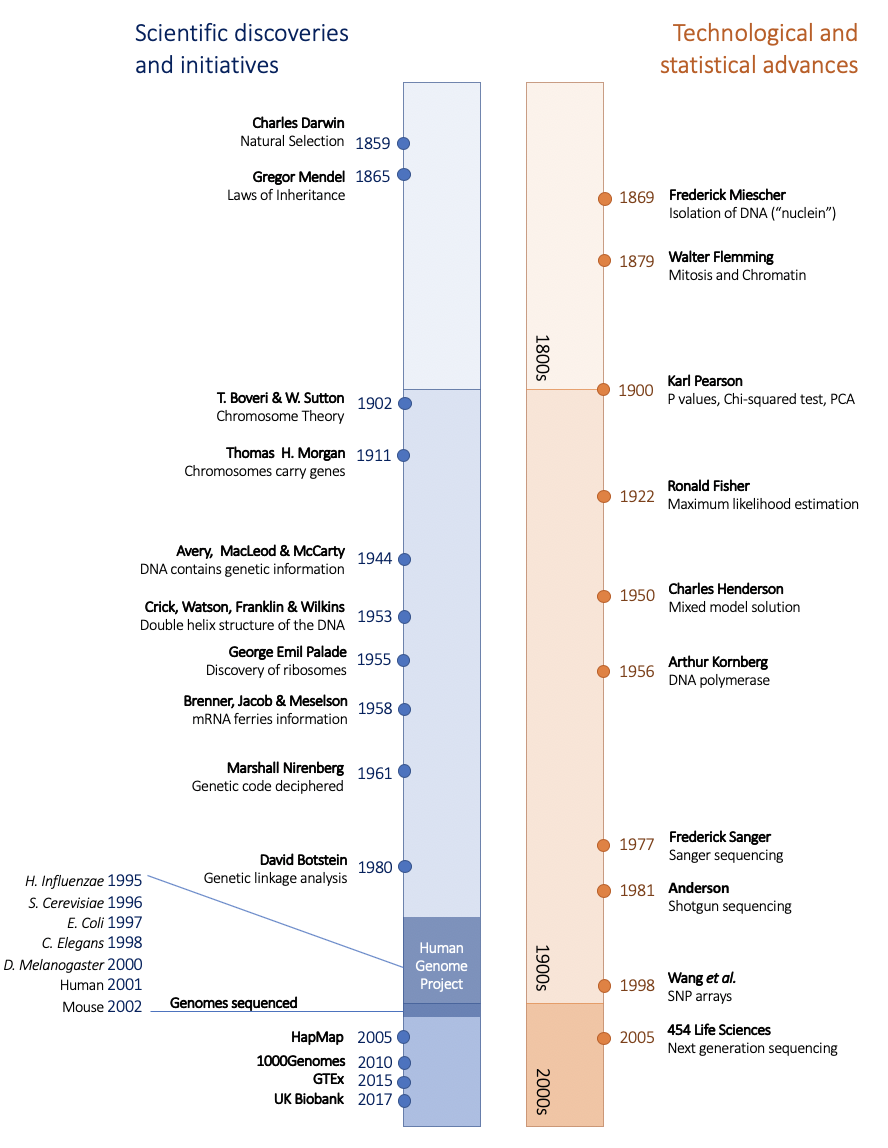
\includegraphics[width=15cm]{Chapter1/Fig/genetic_timeline_draft.png}
\caption[Genetic Timeline]{\textbf{150 years of genetics}.\\
% Key scientific discoveries in genetics and corresponding technological advancements.
A number of scientific discoveries, in combination with key advances in technology and statistical modelling, have led to the identification of thousands of genetic variants which are associated to complex and molecular traits \cite{nhgri2003genetic}.
Several fundamental contributions have been made, from Mendel's peas to the structure of DNA, to large databases cataloguing genetic variation of hundreds of thousands of individuals.
Here, I have attempted to highlight the key events that led to today's field of quantitative genetics in the GWAS and post-GWAS era.}
\label{fig:genetic_timeline}
\end{figure}

\subsubsection{Sequencing DNA}

In terms of technology, one major leap in our understanding of the biological basis of genetic variation was the development of \gls{dna} sequencing, which allowed the nucleotide sequence of a DNA segment to be determined.
In the mid 1970s, two different \gls{dna} sequencing techniques were independently developed: the well known and still used Sanger chain-termination method \cite{sanger1975rapid, sanger1977dna} and a chemical sequencing method that has been almost forgotten, known as Maxam–Gilbert sequencing \cite{maxam1977new}.
The former, named after its developer Frederick Sanger,
% eventually became the standard for \gls{dna} sequencing.
% It 
relies on \textit{in vitro} DNA replication by DNA polymerase,
% the DNA copying enzyme, 
which had been isolated some twenty years prior by Arthur Kornberg and colleagues \cite{kornberg1956enzymic}.
The selective incorporation of chain-terminating dideoxynucleotides (ddNTPs)\footnote{either ddATP, ddCTP, ddGTP or ddTTP.
These chain-terminating nucleotides lack a 3'-OH group required for the formation of a phosphodiester bond between two nucleotides, causing DNA polymerase to cease extension of DNA when a modified ddNTP is incorporated - thus the name chain-terminating sequencing.} alongside regular nucleotides during DNA synthesis, and the use of polyacrylamide gel electrophoresis to separate the resulting fragments allows
% Using a primer to recruit the DNA polymerase, four reactions are performed (one per nucleotide).
% In each reaction numerous deoxinucleotides (dNTPs)\footnote{i.e. dATP, dCTP, dGTP, dTTP.} are included to allow DNA synthesis, while only one type of dideoxinucleotide (ddNTP)\footnote{either ddATP, ddCTP, ddGTP or ddTTP.} is included, in much smaller concentrations.
% The ddNTP terminates the synthesis DNA polymerase, thus the name chain-termination.
% Next, the reactions contents are loaded into four separate lanes of a 
% % polyacrylamide 
% gel and the fragment separate by size by electrophoresis, allowing
the sequence of an input DNA fragment to be determined. \\

% The former (named after its developer Frederick Sanger)
Sanger sequencing eventually became the standard for \gls{dna} sequencing, and
% In the next years, 
subsequent innovations led to the development of automatic sequencing machines able to sequence DNA fragments of about one kilobase (kb) in length. 
For sequencing longer stretches of \gls{dna}, a novel strategy named `shotgun sequencing' was developed \cite{staden1979strategy, anderson1981shotgun}. 
In shotgun sequencing, the long \gls{dna} of interest is randomly broken up into shorter \gls{dna} fragments which are cloned and sequenced separately. 
The occurrence of overlapping \gls{dna} fragments 
% given by the random nature of creating the short fragments
allows for the \textit{in silico} reconstruction of longer \gls{dna} fragments. \\

% The next year (1976) the first genetic engineering company, Genentech, was founded by Herbert Boyer and Robert Swanson. 
% Restriction enzymes as scissors
% shotgun, insulin (?)\\


% 1983: PCR (polymerase chain reaction) is invented 

 
In 1995, the first genome of a living organism (the bacteria \textit{Haemophilus influenzae}) was sequenced and assembled by shotgun sequencing \cite{fleischmann1995whole}, shorty followed by that of another bacterium, \textit{Mycoplasma genitalium} \cite{fraser1995minimal}. 
The genomes of other model organisms were to follow in subsequent years - the budding yeast \textit{S. cerevisiae} \cite{goffeau1996life}, the bacterium \textit{E. coli} \cite{blattner1997complete}, the worm \textit{C. elegans} \cite{c1998genome}, the bacterium \textit{M. Tuberculosis} \cite{cole1998deciphering}, the fruit fly \textit{D. melanogaster} \cite{adams2000genome} and the flowering plant \textit{Arabidopsis taliana} \cite{kaul2000analysis}.
The first two human chromosomes (chromosome 22 and chromosome 21) were sequenced in 1999 and 2000, respectively \cite{dunham1999dna, hattori2000dna}, and the first draft of the entire human genome was published in 2001 \cite{lander2001initial, venter2001sequence} (see \textbf{section \ref{sec:hgp}}).
The mouse genome was only published in 2002 \cite{waterston2002initial}.

\subsubsection{Understanding the genetic basis of disease}
% \subsubsection{Mapping genotype to disease}

In parallel, along with the increasing understanding of the molecular structure of genes and the genome, scientists began to investigate the molecular basis of disease.
One of the first conditions to be linked to a genetic cause was alkaptonuria\footnote{a rare recessive condition that affects mainly the joints and causes unusual pigmentation.}, which in 1902 Garrod had identified  to follow the Mendelian rules of inheritance \cite{garrod1902incidence}.
In 1956, Vernon Ingram for the first time traced the cause of a disease to a genomic alteration: he discovered that sickle cell disease (SCD) is caused by a chemical change in a hemoglobin protein \cite{ingram1963hemoglobins}.
% A few years later, in 1959, Jerome Lejeune and colleagues identified Down Syndrome to be caused by trisomy 21, that is the presence of three copies, rather than two, of chromosome 21 \cite{lejeune1959etude}.
% 1961: Screen for metabolic defect (Guthrie)
\\

Until the 21st century, success in identifying genetic factors responsible for human traits and diseases was predominantly 
% for monogenic disorders 
through the use of genetic linkage studies, first proposed in 1980 by David Botstein \cite{botstein1980construction}.
These rely on the concept of linkage, first introduced by Morgan and his students: during meiosis, physically close genes remain `in linkage', whereas genes that are further apart are less likely to co-segregate due to recombination events.
When analysing a disease segregating\footnote{recurring within a family but without affecting all of its members.} in a family, linkage analysis
% was a laborious method that 
involves i) identifying a genetic marker (with a known location) that is linked to the (unknown) disease gene and then ii) testing each of the nearby genes to determine the one that causes disease \cite{teare2005genetic}. 
% from Rachel's thesis
% Genetic linkage relies on a definitive phenotype repeatedly occurring within a family that does not affect all members (segregation) and that during meiosis, physically close genes remain in linkage whilst those that are further apart are less likely to co-segregate due to recombination events. 
% This enables, with the use of genetic markers (approximately spaced uniformly along the genome), identification of genomic regions that are co-inherited in diseased individuals more often than is expected by chance that are not co-inherited in non-diseased individuals. 
% The allelic configuration of a set of genetic markers along a single chromosome (or a section of a chromosome) is defined as a haplotype and as result diseased individuals will share the same haplotype at the co-inherited genetic markers.
Using this method, in 1983, the first disease gene was mapped, when Gusella and colleagues linked a gene on chromosome 4 to Huntington's disease \cite{gusella1983polymorphic}.
Shortly after, in 1989, there followed a study from Francis Collins and others, identifying the genetic basis of cystic fibrosis as a single base deletion on chromosome 7 \cite{riordan1989identification}.
As of 2003, about 1,200 genes were linked to Mendelian traits \cite{botstein2003discovering}.\\

Mendelian disorders, as the name suggests, are those that follow the Mendelian laws of inheritance.
They are often called monogenic, as they are typically driven by mutations within a single gene with high penetrance (defined here as the probability of having a trait/disease given the predisposition score). 
Examples of such traits include X-linked muscular dystrophies, cystic fibrosis, Fanconi anaemia and phenylketonuria. 
Mendelian traits are typically rare 
% (low frequency) 
in the general population but often cluster in families.
Genetic linkage analyses are best powered to discover these highly penetrant monogenic disease genes \cite{cardon2001association}.\\

% Candidate gene analysis (Tabor et al., 1988). \cite{tabor2002candidate}
% To perform such an analysis, researchers would perform genotyping in and near a gene with a plausible role in the disease of interest, and then test for variant-phenotype associations in a collection of affected individuals and controls.

% from here onwards this section needs more references
% Ever since the biometric-mendelian debate, ..
% It is widely accepted today that the genetic architecture of human disease is captured on a spectrum \cite{manolio2009finding} and can be broadly categorised as Mendelian (monogenic), complex (polygenic) or chromosomal. 
% The genetic architecture of monogenic and multifactorial disease can typically be described by the frequency and penetrance of disease-associated variants.\\

% Sara
In comparison, complex traits are typically common in the general population\footnote{The genetic architecture of human disease is captured on a spectrum \cite{manolio2009finding} but can be broadly categorised as i) Mendelian (monogenic), ii) complex (polygenic) or iii) chromosomal.}.
They are driven by a combination of multiple genetic risk factors across the genome (thus the name polygenic), environmental risk factors, as well as interaction effects between genetic variants and environmental exposures (GxE).
These common, multifactorial diseases have a genetic architecture that is highly distinct from that of monogenic disease. 
They are known to be heritable (heritability estimates for most common diseases are estimated at 40-60\% \cite{manolio2009finding, prokopenko2009variants, kathiresan2008six, zeggini2008meta, harley2008genome}), but their full etiology contains both a genetic and an environmental component.
Consequently, it is the cumulative effect of many subtle genetic variants and environmental risk factors that, working in concert, trigger disease onset.
% Complex traits include quantitative traits, such as height, weight and blood pressure and complex diseases typically modelled as binary outcomes (i. e. either diseased or not). 
Complex diseases include heart disease, type 2 diabetes, asthma, cancer, schizophrenia and Parkinson's disease.\\

Whilst there was some success in using linkage studies to identify genetic regions involved in complex traits and diseases\footnote{For example BRCA1 for breast and ovarian cancer  \cite{bailey2011linkage, miki1994strong}.},
% including NOD2 for inflammatory bowel disease34-38 and BRACA1 for breast and ovarian cancer38,39, 
% the relative lack of success implied that the genetic mechanisms responsible for complex diseases were different to those responsible for rare disorders26 and  that, as a consequence, 
genetic linkage studies in general proved underpowered to detect regions with significant linkage for complex traits and diseases \cite{bush2012genome, altmuller2001genomewide}. 
This was in line with the `common disease/common variant' (CD/CV) hypothesis \cite{bush2012genome, reich2001allelic}, which postulated that common traits are driven by genetic variation that is common in the population, i.e. multiple variants, each with low penetrance.
% If true, based on the population prevalence of complex traits, the effects of these variants would be small relative to the effects observed for rare variants[26]. 
% Consequently, to explain the estimated heritability (estimated fraction of phenotypic variation explained by genetics44,45) of such common traits, many genetic variants must influence complex disease susceptibility26.
This hypothesis was described as early as 1996, and had already suggested that family-based linkage studies would be underpowered to detect variants with modest effects \cite{risch1996future}. \\

Instead, it was proposed that the combined use of \gls{ld}\footnote{LD: the nonrandom allocation of alleles at nearby variants to individual chromosomes as a result of recent mutation, genetic drift or selection, manifest as correlations between genotypes at closely linked markers \cite{mccarthy2008genome}. 
% % Rachel
% the observed departure from the expected co-occurrence of two genetic markers based on their observed frequencies (i. e. non-zero correlation between the two genetic markers)
% % Sara
% the correlation between genetic variants that typically reside close to one another in the genome and are inherited in blocks or haplotypes.
} and population- (rather than family-) based studies would be more suitable \cite{risch1996future, jorde2000linkage} - thus practically proposing the design for \glspl{gwas} \cite{risch1996future}.
However, at the time, implementation of \glspl{gwas} was not possible, for two primary reasons.
First of all, the technology required to genotype thousands to millions of markers in a single experiment for the larger required sample sizes was not available \cite{risch1996future, visscher2012five}.
Secondly, the distribution and density of genetic polymorphisms across the genome, and the \gls{ld} between genetic variants across different populations, were unknown.\\

In some sense, population-based association studies can be viewed as an extension of family-based linkage studies, in which the population studied (derived from common ancestors) acts as an extended pedigree and a much greater number of meiotic recombinations will have occurred between the analysed samples.
As a consequence, \gls{ld} regions are much smaller than within pedigrees of close relatives, thus requiring that a more dense panel of genetic markers be examined \cite{cordell2005genetic}.

\subsubsection{The Human Genome Project}
\label{sec:hgp}

In order to study genomic variation, it was necessary to generate a reference genome.
% in the US started by Jim Watson and then led by Francis Collins (since 1993)
% and then Celera (Craig Venter, 1998)
% in the UK (at Sanger) by first John Sulston (first worm sequenced), and then Jane Rogers\\
% A driving force behind the growth and success of genetic association studies has been technological evolution,
% ; breakthroughs in \gls{dna} sequencing and genotyping have
% which has
% pushed human disease research forward, inducing a shift in the field each time new advances were introduced. 
This was the goal of the \gls{hgp}, which aimed at sequencing the entire human genome.
The \gls{hgp} was perhaps the first major breakthrough to dramatically change the landscape of genetics, and was described by United States President Clinton as “an epic-making triumph of science and reason” \cite{clinton2000remarks} at the announcement of its completion.
Driven by and driver of technological breakthroughs in \gls{dna} sequencing and genotyping, the \gls{hgp} was a massive international undertaking and a truly collaborative effort; sequencing and analysis took place across twenty centers in six different countries (USA, UK, France, Germany, Japan, China) and took 13 years to complete, costing approximately \$2.7 billion \cite{lander2011initial}.
% Led by then NIH director Francis Collins and founder of Celera Genomics\footnote{The company Celera Genomics was formed in May 1998, with the objective of sequencing much of the human genome in three years
% % . Celera used a shotgun sequencing strategy, in which the entire genome is fragmented and random segments are sequenced and then put in order 
% \cite{venter1998shotgun}.} Craig Venter, the \gls{hgp} was announced by the White House in 2000.
Led in the US by then NIH director Francis Collins and by founder of Celera Genomics\footnote{The company Celera Genomics was formed in May 1998, with the objective of sequencing much of the human genome in three years
% % . Celera used a shotgun sequencing strategy, in which the entire genome is fragmented and random segments are sequenced and then put in order 
\cite{venter1998shotgun}.} 
Craig Venter, and with large contributions from the UK, in particular from the Sanger Institute directed by John Sulston (who had first sequenced the genome of \textit{C. Elegans}), the \gls{hgp} was announced as a joint US-UK statement on June 26th, 2000.
After a first publication in 2001, the project was truly completed on April 25th, 2003, on the 50$^{th}$ anniversary of the Watson and Crick paper describing the helical structure of \gls{dna}.\\

The \gls{hgp} provided the first map (obtained from the genomes of a small number of individuals) of the $\sim$3 billion bases in the human genome \cite{lander2001initial, schmutz2004quality, hattori2005finishing}, and revealed that human \gls{dna} consists of surprisingly few exons (1.1\% of the genome), whereas introns cover 24\% of the genome \cite{venter2001sequence, lander2001initial}. 
Additionally, the number of genes was found to be smaller than expected, with around 30,000 being identified in 2001, and circa 21,000 genes being the latest (still debated) estimate at the time that this thesis is written \cite{pertea2018thousands}. 
Additional breakthroughs in sequencing technologies have expanded and refined the reference genome, which now captures more than 92\% of the genome and provides a landscape of its 
% 20,000 
genes \cite{lander2011initial}.\\

With a complete map of the human genome in place, genetic variants could now be identified as those bases discovered in an individual that did not match the (reference) base annotated in the human genome map. 
Common variants, i.e. variants with \gls{maf}\footnote{The frequency of an
allele at a genetic variant is the proportion of chromosomes in the population that
carry that allele \cite{laird2010fundamentals}. 
For a biallelic variant (a variant for which only two possible alleles are observed in the population), the frequency of the less common allele (minor allele) is called the minor allele frequency (MAF).} larger than 5\%, were called \glspl{snp}. 
Previous studies had estimated that approximately 0.1\% (1 base per 1,000) of an individual's genome was a polymorphism \cite{wang1998large, li1991low, cargill1999characterization}. 
% Most of these polymorphisms were scattered across the genome and no one had yet broadly described what these variants were, where in the genome they resided, and what (if any) phenotypic effect they conferred.

\subsubsection{The International HapMap Project}

The International HapMap Project was the first effort of its kind to systematically catalogue genomic variation. 
Additionally, it aimed to characterise the LD structure of the human genome, which would make \glspl{gwas} feasible. 
The HapMap was officially started in October 2002 as a collaboration between research groups and private companies in Canada, China, Japan, Nigeria, the United Kingdom and the United States with the aim to develop a haplotype map (HapMap) of the human genome \cite{international2003international}.
By genotyping individuals of African (YRI), European (CEU) and East Asian (JPT, CHB) descent, in Phase I HapMap assembled a publicly available database of common variants (\gls{maf}>5\%) in global samples \cite{international2005haplotype}. 
The HapMap expanded rapidly. 
By Phase II (2007), the database contained 2.1 million SNPs from the four original populations \cite{international2007second}.
Phase III (2010) added genotyping from seven additional populations, for a total of over 3 million SNPs in 11 global ancestry groups\footnote{ASW (African ancestry in Southwest USA); CEU (Utah residents with Northern and Western European ancestry from the CEPH collection); CHB (Han Chinese in Beijing, China); CHD (Chinese in Metropolitan Denver, Colorado); GIH (Gujarati Indians in Houston, Texas); JPT (Japanese in Tokyo, Japan); LWK (Luhya in Webuye, Kenya); MEX (Mexican ancestry in Los Angeles, California); MKK (Maasai in Kinyawa, Kenya); TSI (Tuscans in Italy); YRI (Yoruba in Ibadan, Nigeria).} \cite{international2010integrating}.\\ 

% With the map of the genome complete and cataloguing efforts moving apace, researchers could now begin to search for modest effect genetic variants associated to human disease across the full length of the genome.\\

% % 1000 genomes

% % Sequencing technologies have provided the field with an opportunity to expand the catalogue
% % of human genetic variation. Similar to the HapMap initiative, The 1000 Genomes
% % Project (1KG) (Abecasis et al., 2012) was started with the aim of cataloguing human
% % variation in global populations down to alleles with a minor allele frequency of 1%.

The growing popularity of genetic association studies in parallel with the expansion of the HapMap effort paved the way for the last needed technological breakthrough: microarrays.
By knowing the genetic location of thousands of variants, commercial companies were able to develop so-called `SNP chips' \cite{meaburn2006genotyping, oliphant2002beadarray}, which allowed for genotyping at specific locations across the genome.
% With input from the academic community, the company Affymetrix released the GeneChip Human Mapping 100K Set (Meaburn et al., 2006), designed to allow for agnostic interrogation of SNPs and copy number variants (CNVs) across the genome; Illumina developed BeadArray technology (Oliphant et al., 2002), also allowing for genome-wide capture of thousands of SNPs.
In parallel, the data generated by the HapMap project enabled calculation of the LD\footnote{Pearson's correlation coefficient squared, $r^2$, is commonly used} between SNPs within the genome, effectively describing the chance that two SNPs will be inherited together \cite{bush2012genome}.
This enabled the identification of haplotypes and thus a minimal set of SNPs that capture the majority of the haplotype diversity 
% (common variation) 
within a population, known as `tag SNPs' \cite{international2003international}. 
Tag SNPs are population specific, with approximately 500,000 variants in Europeans and up to one million variants in non-Europeans required to capture > 80\% common variation (MAF > 5\%) with LD, $r^2$ > 0.8 \cite{bush2012genome, visscher2012five}.
% These tag variants are used to conduct indirect association studies, where associations are tested for only at the tag variants. 
% As a result, any identified significant associations can be due either to the tested tag SNP or caused by a variant that is in high LD with the tested tag variant. 
% Indirect association studies are much cheaper than conducting direct association studies, where association at each common SNP is tested for26,48. 
% Using such tagging SNPs, reduces the genetic region associated with a trait to approximately 10-100 kb (which is often just a few genes) from the 5-10 Mb (which can contain tens to hundreds of genes) regions that were identified with genetic linkage studies[8].
% In parallel, researchers continued to gather information on genetic recombination hotspots and linkage disequilibrium (LD) (Wegmann et al., 2011; Lynn et al., 2004; Slatkin, 2008; Smith and O'Brien, 2005;), the correlation between genetic variants that typically reside close to one another in the genome and are inherited in blocks or haplotypes. 
The collective LD information gathered by academics in those years \cite{slatkin2008linkage, pe2006evaluating, otto2002resolving} allowed companies such as Affymetrix and Illumina to develop SNP arrays that contained 
these tag SNPs,
% SNPs with many `tagging' SNPs in high linkage disequilibrium, 
effectively capturing information about common variation 
% (minor allele frequency >5\%) 
across a large percentage of the genome while only directly genotyping a few thousand SNPs.\\

\newpage

% % %********************************** % 1.1.7  **************************************
\subsection{Genome-wide association studies}
\label{sec:gwas}

% from Sara's thesis, rewrite
The sequence of the human genome, the development of faster, massively-parallel next-generation sequencing techniques, 
% (reviewed in [Shendure et Ji, 2008; Heather et Chain, 2016]) 
and \gls{dna} microarrays that allow for the genotyping of hundreds of thousands of genetic markers simultaneously \cite{wang1998large}, started a new era of human genetic and genomic research.
In particular, the data generated by the International HapMap Project combined with development of appropriate chip-based microarray technology, which enabled simultaneous genotyping of more than one million SNPs, led to the first wave of \glspl{gwas} \cite{visscher2012five}.
\gls{gwas} are a hypothesis-free\footnote{bar the selection of SNPs on the chip. 
More recently, shallow DNA-seq has been increasingly used as an alternative, making the approach truly hypothesis-free.} approach to test for statistical association between the genotype frequency of common genetic variants (considered one by one across the genome) and a phenotype of interest \cite{mccarthy2008genome}. \\

Initially, \gls{gwas} focused on complex phenotypes with binary outcomes, using a case-control design (i.e. diseased vs healthy).
Then, for each SNP and binary trait, the association was evaluated using a Cochran–Armitage (trend) test, a $\chi^2$ test or a Fisher's exact test comparing the numbers of cases and controls when stratified by their alleles at the locus of interest. 
The first successful \gls{gwas} was published in 2002 on myocardial infarction \cite{ozaki2002functional}.
The same design was then applied in a landmark GWA study conducted in 2005 for age-related macular degeneration (AMD), using 96 cases and 50 healthy controls and testing for associations at $\sim$100,000 SNPs \cite{klein2005complement}. 
In 2007, the Wellcome Trust Case-Control Consortium (WTCCC) published a study where they performed \gls{gwas} on seven different common diseases, using a common set of 3,000 healthy controls and 2,000 cases for each of bipolar disorder (BD), coronary artery disease (CAD), Crohn's disease (CD), hypertension (HT), rheumatoid arthritis (RA), type I and II diabetes (T1D, T2D) \cite{wellcome2007genome}.\\

A year later, in 2008, the \gls{gwas} Catalog was founded to keep a record of all published \gls{gwas} and identified associations \cite{welter2014nhgri}.
% keep up to date (https://www.ebi.ac.uk/gwas/search, Catalog stats)
% figure out where to find the number of traits
As of August 2020, when I am writing this thesis, the \gls{gwas} Catalog includes 4,671 publications, describing 196,813
SNP-trait
associations
\cite{macarthur2017new}.\\
% between 133,739 genetic variants and XX traits or diseases.\\
% % \gls{gwas} Catalog was founded by \gls{nhgri} in 2008
% % and has become a collaborative project between the \gls{nhgri} and the \gls{ebi} since 2010
% % \gls{gwas} Catalog publications: https://www.ebi.ac.uk/gwas/docs/related-resources\\


% Add (statistical) imputation?\\
% % Whilst these early \gls{gwas} were based on the directly genotyped tag SNPs, from 2008 onwards, utilisation of methods to fill in missing genotype data became increasingly common practice, referred to as imputation (ref). 

% % Imputation is a statistical technique to infer genotypes. 
% % The general idea is to compare genotyped samples to a reference panel of individuals of similar ancestry to identify short haplotype stretches that are shared between the genotyped and reference samples (Fig. 1.3b). This then allows missing genotypes to be filled in.
% % Initially, data from the HapMap Project was used as a reference panel, with for example the CEU panel used to impute samples of European ancestry. 
% % Imputation is now also used to explore association effects of rare variants (see Section 1.2.1 for further details of imputation of rare variants, including examples of current reference panels used).
% Statistical imputation5, 6, 7 of unobserved variants can recover some of the information lost because of imperfect LD between observed genotypes and unobserved causal variants. Imputation is enabled by the fact that the genotypes of unobserved genetic variants can be predicted by the haplotypes inferred from multiple observed SNPs and the haplotypes observed from a fully sequenced reference panel.

Over time, quantitative traits have become increasingly popular to use as phenotypes, in addition to binary traits.
These include continuous traits such as height, weight and blood pressure.
% % % This is partly due to the fact that the onset of many diseases is time dependent, meaning that some individuals selected as controls may later become cases and hence the control group actually contains a mixture of cases and controls, resulting in some loss of power. 
% % % In addition, some binary traits are defined by thresholding a continuous variable, with the threshold somewhat arbitrary such that an individual with a value marginally greater than the cutoff is said to be `diseased' whilst an individual just below the threshold is defined as `healthy'.
% % % Examples include defining obesity based on a BMI threshold and diabetes based on fasting glucose levels. 
% % % This thresholding approach results in loss of information regarding phenotypic similarity and as a result, using the binary outcome is likely to be less powered than using the underlying quantitative trait. 
% % % Moreover, quantitative traits are often closer to the underlying biology, providing greater insight into the mechanisms underpinning trait or disease development and the results from using continuous traits may be more directly interpretable, in that it is possible to quantify the average difference in trait outcome per risk allele carried.
Furthermore, linear regressions and their derivations have become more popular methods to assess association, due to their flexibility to include covariates \cite{mccarthy2008genome}.
I describe these models in detail in the next chapter (\textbf{Chapter 
% 2
\ref{chapter2}}). 

\newpage

\gls{gwas} results are often visualised using Manhattan plots \cite{mccarthy2008genome}, with the negative log p value plotted on the y-axis against the corresponding genomic position (ordered by chromosome and position) on the x-axis (\textbf{Fig. \ref{fig:manhattan}}). 
Peaks on these plots represent loci (multiple variants in \gls{ld}) that display evidence of association with the analysed phenotype. 
Variants are deemed to be significantly associated with a trait if they exceed an appropriately chosen p value threshold. 
% \\
% Due to \gls{ld} structure, if a peak arises from a single variant, this is usually indicative of a false positive finding. 

\begin{figure}[h]
\centering
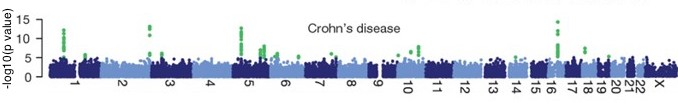
\includegraphics[width=15cm]{Chapter1/Fig/Manhattan_plots_CD_WTCCC_2007.jpg}
\caption[Manhattan plot]{\textbf{Manhattan plot}.\\
Manhattan plot for Crohn's disease (CD) from the WTCCC study \cite{wellcome2007genome}.
On the x axis are plotted the genomic positions of the SNPs tested, one chromosome after the next.
On the y axis are the association significance values.  
Alternating colours are used to distinguish chromosomes (odd numbered chromosomes -and chromosome X- are dark, even light).
Highlighted in green are statistically significant SNPs (p value < $5 \times 10^{-8}$).}
\label{fig:manhattan}
\end{figure}

% % \newpage
% % %%%% Box on GWAS terms

% \begin{Comment}
% \hspace{-2.5mm}\textbf{Box 2: GWAS glossary}\label{box:gwas}
% \small
% \begin{itemize}
%     \item \textbf{Linkage disequilibrium (LD)}: the nonrandom allocation of alleles at nearby variants to individual chromosomes as a result of recent mutation, genetic drift or selection, manifest as correlations between genotypes at closely linked markers \cite{mccarthy2008genome}. 
%     \item \textbf{Hardy-Weinberg equilibrium (HWE)}: a theoretical description of the relationship between genotype and allele frequencies that is based on expectation in a stable population undergoing random mating in the absence of selection, new mutations and gene flow: in the context of genetic studies, departures from equilibrium can be used to highlight genotyping errors \cite{mccarthy2008genome}.
% \end{itemize}
% \vspace{3mm}
% \end{Comment}

% \vspace{3mm}

% \subsubsection{From case-control to cohort studies}

% A first effort to ...
% was the 1000 Genomes project

% The 1000 Genomes Project ran between 2008 and 2015, creating the largest public catalogue of human variation and genotype data.
% The final dataset contains data for 2,504 individuals from 26 populations.\\

% % pilot: 2010 \cite{10002010map}
% % phase 1: 2012 \cite{10002012integrated}
% % phase 3: 2015 \cite{10002015global, sudmant2015integrated}\\

% The UK Biobank is a massive... consisting of over 500,000 individuals \cite{bycroft2018uk}..

% similar studies in the US, estonia, finland, the netherlands

% Nevertheless, now hundreds of thousands of genomes are being sequenced as part of major initiatives, and the next 5 years will allow direct comparisons of discoveries made from sequencing and array studies. 

% Reviews:

% Goals of GWAS (2005) \cite{hirschhorn2005genome}

% 5 years of GWAS (2012) \cite{visscher2012five}

% 10 years of GWAS (2017) \cite{visscher201710}
% \\


% Successful examples of elucidated mechanisms:

% KLF14 for metabolic pathways \cite{small2011identification}

% FTO obesity

% MHC schizophrenia


% \subsubsection{Challenges in GWAS}

% polygenic/omnigenic architecture - the missing case of heritability \cite{manolio2009finding}
% Many traits of interest are complex and can be regulated by tens or even hundreds of genetic loci with each locus having a small individual effect (Wood et al., 2014; Ripke et al., 2014).\\
% % \\
% Moreover, genetic variants commonly entail pleiotropic effects across several related phenotypes and diseases (Fortune et al., 2015; Pickrell et al., 2016) and interactions of genetic effects with environmental factors and other contexts are common (Andreassi, 2009; Winkler et al., 2015). 
% Additionally, many discovered
% variants lie in non-coding regions of the genome, hampering the interpretation
% of the molecular mechanisms that underlie such associations.

% % additive - omnigenic model \cite{boyle2017expanded}\\
% % % % \cite{timpson2018genetic} review on genetic arch.

% % population used - europeans only?\\

% Rare diseases: often rare variants too (\gls{maf}<0.05)
% Pleiotropy: same variant affects multiple traits

% non-additive interactions:
% Epistasis: combined effect of separate variants interacting to have an effect on trait
% GxE:interaction between a variant and an environment\\

% Genetic studies of gene expression levels and other molecular traits have helped identify the regulated gene for a fraction of such intergenic GWAS loci. 
% However, as the effects of genetic variants can arise in specific tissue types or under specific stimuli (GTEx Consortium, 2015; Fairfax et al., 2014), these genetic studies need to be conducted in disease-relevant cellular types and states.

% % % \subsection{Genotype-Environment interactions}

% % % Explicitly, whilst a variant with a significant genetic effect is determined by a mean phenotypic difference between groups of individuals with different allele dosages and a significant environment effect is determined by a mean phenotypic shift that is constant across different allele dosages (Fig. 1.6b), a significant statistical interaction effect is defined when there is a significant difference in the genetic effect between two groups of individuals with different environmental exposures.

% % % % \begin{figure}[h]
% % % % \centering
% % % % 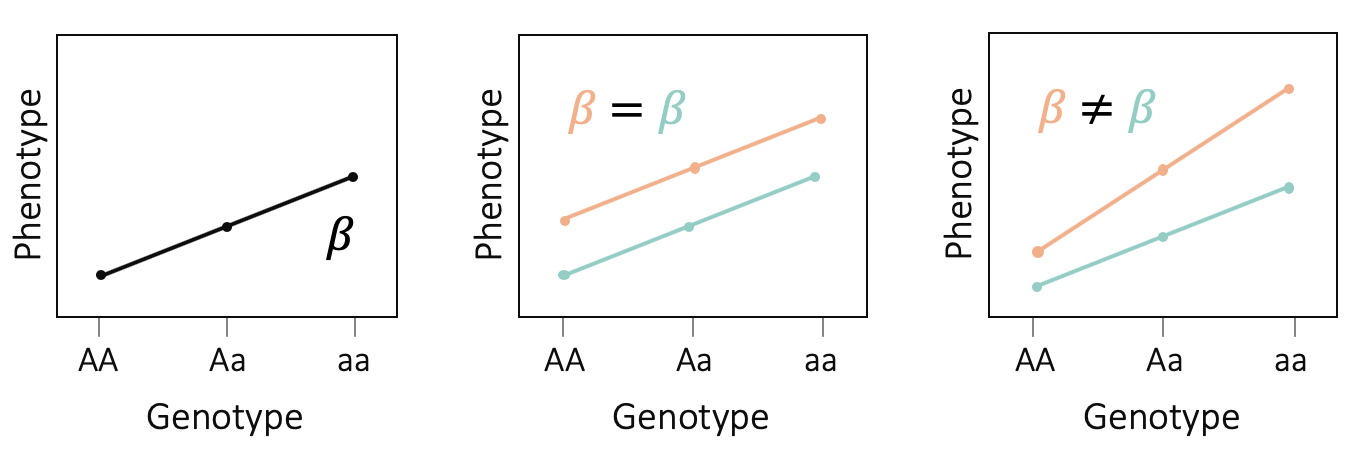
\includegraphics[width=15cm]{Chapter1/Fig/GxE.png}
% % % % \caption{\textbf{Illustration of GxE effect}.\\
% % % % a) Genetic effects only. b) Environments have effects on phenotype but do not change the genetic effect. c) Interaction effect between genotype and environment (GxE).}
% % % % \end{figure}

% % % \newpage

% % \begin{figure}[h]
% % \centering
% % 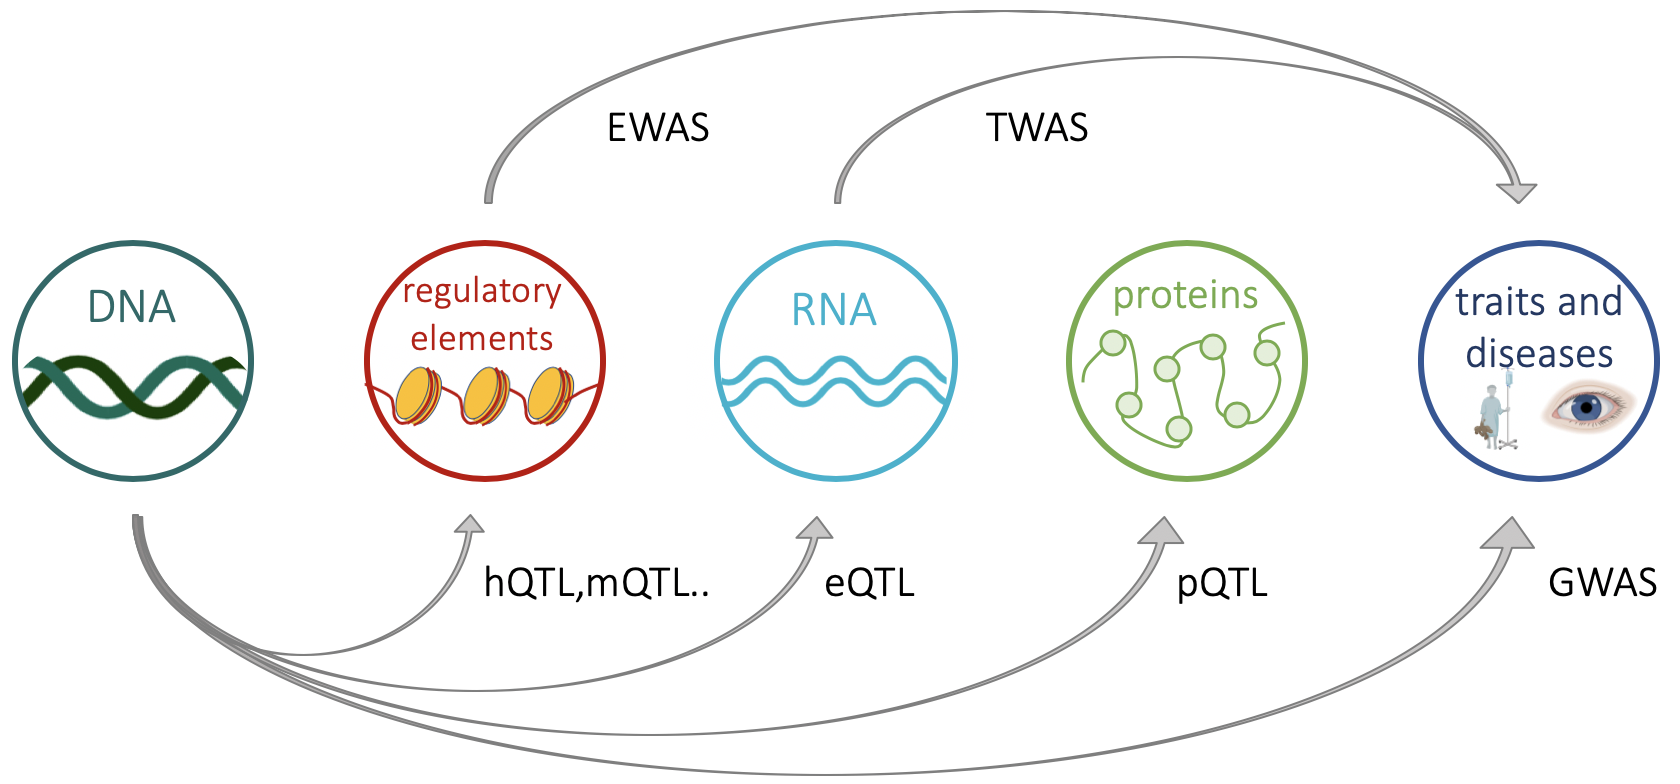
\includegraphics[width=15cm]{Chapter1/Fig/layers_of_genetic_associations_draft.png}
% % \caption[Genetics of molecular and global traits]{\textbf{Genetics of molecular and global traits}.\\
% % Layers of genetic association analyses to understand the molecular mechanisms underpinning the genotype-phenotype map}
% % \label{fig:molecular_genetic_associations}
% % \end{figure}

% % \newpage

\subsubsection{From global traits to molecular traits}

The path from \gls{gwas} to biology is not straightforward, because an association between a genetic variant at a genomic locus and a trait is not directly informative of the causal mechanisms whereby the variant is associated with phenotypic differences \cite{visscher201710}. 
\gls{gwas} have robustly associated thousands of genomic loci with complex traits. 
Despite this success, \gls{gwas} loci are often difficult to interpret - LD often obscures the causal variants driving the association, and the causal genes mediating variant effects on the trait are rarely ascertainable from \gls{gwas} data alone, especially for non-coding variants, which account for the majority of \gls{gwas}-identified risk alleles \cite{manolio2009finding, gallagher2018post, wainberg2019opportunities}. 
% \\
Maps of regulatory annotations and connections in disease-relevant tissues, generated by projects such as ENCODE (ENCyclopdia Of DNA Elements, \cite{encode2004encode}) and Epigenome RoadMap \cite{kundaje2015integrative} can help the interpretation of these (putative) regulatory variants.
Additionally, molecular quantitative trait loci (QTL) mapping, where genomic variants are associated with changes in expression (eQTL \cite{schadt2003genetics}), DNA methylation (mQTL \cite{gaunt2016systematic}), histone modifications (hQTL \cite{grubert2015genetic}) or protein (pQTL \cite{melzer2008genome}) level, have added an interpretative layer to the molecular mechanisms associated with disease-associated variants.
\\

In this thesis, I focus on gene expression, i.e., the transcriptome, as a molecular phenotype.
I use the next section (\textbf{section \ref{sec:eqtl}}) to describe key aspects of eQTL mapping.

% the decrease in cost of high-throughput profiling of gene expression has made it possible to measure gene expression levels in large numbers of individuals, thereby enabling the mapping of quantitative trait loci for gene expression (eQTL mapping, \cite{schadt2003genetics}). 
% More recently, these studies have been extended to test for genetic effects on different regulatory elements, including DNA methylation (mQTL, \cite{gaunt2016systematic}), histone modifications (hQTL , \cite{grubert2015genetic}) as well as the activity of known proteins and protein complexes that regulate expression and chromatin accessibility, such as transcription factors 
% % ( \cite{was} (Waszak et al., 2015).
% pQTL \cite{melzer2008genome}
% % Additionally, molecular \glspl{qtl}

% % %********************************** % 1.1.8  **************************************
\subsection{Expression quantitative trait loci}
\label{sec:eqtl}

% % Nils Koelling
% Despite the additional level of resolution provided by GWAS, the complex genetic mechanisms that underlie whole-organism phenotypes have proven challenging to understand. 
% Exactly how loci identified in a GWAS affect the phenotype often remains an open question, especially as many of them are not located inside protein-coding regions (for example Easton et al., 2007).

% It thus stands to reason that many of the loci identified in GWAS do not affect the amino acid composition of a protein, but instead change the expression level of genes through changes in gene regulatory regions. 
% This change in gene expression level could then in turn affect the phenotype.
% Understanding the effects of mutations on gene expression levels is thus an important step towards bridging the gap between genotype and phenotype.
% With the decreasing cost of microarrays and later RNA-seq (see Section 1.4), it has now become possible to measure the expression levels of all genes of an organism in a high-throughput manner. 
% By considering these measurements of gene expression levels as quantitative traits, a QTL study on gene expression can be performed for each individual gene using a single assay. 


% To circumvent this problem, eQTL studies often restrict the set of variants to be tested to those in close proximity to the gene. 
% This is based on the assumptions that most \textit{cis} regulatory regions are located near the gene and that changes to \textit{cis}-acting gene regulation have larger, more easily detectable effects than changes to trans-acting gene regulation (Petretto et al., 2006; Wittkopp and Kalay, 2011).


\subsubsection{Regulation of gene expression}

During gene expression (or transcription), the genetic information stored in restricted portions of the \gls{dna} (genes) is used to produce 
% molecular products. 
% The information on the composition of these products is contained in restricted portions of the genome known as genes. 
% In the first step of gene-expression (transcription), genes are transcribed into 
\gls{rna} molecules. 
% Although RNA molecules can be the final product of gene expression, many 
Next, during translation, the majority of RNA molecules are translated into  proteins 
which are
% in a process known as translation. Proteins are 
long chains of smaller molecules called amino acids. 
As we have seen, only approximately 1.5\% of the human genome codes for proteins \cite{lander2001initial} while a large fraction of the remaining portion is likely to play a role in the regulation of gene expression \cite{encode2004encode}. \\

The impact of genetic variation on traits and disease is the consequence of perturbations to this complex molecular machinery.
An easily interpretable mechanism through which genetic variants may affect a phenotype is the direct alteration of the sequence 
% - or structure -
and therefore functionality of the coded protein \cite{westra2014genome}. 
As an example, sickle cell anaemia is caused by a \gls{snp} in the \textit{HBB} gene, which causes a substitution of an amino acid in the sequence of the coded protein \cite{laird2010fundamentals}. 
Alternatively, genetic variation may affect the regulation of gene expression. 
One way this can occur is through the disruption of a specific sequence that affects the binding of
proteins regulating the expression of a gene, 
% an expression-regulating protein, 
for example 
% e.g.
a \gls{tf}. 
In this scenario, the regulatory variant is said to be acting in \textit{cis}.
Another possibility is the alteration of the structure of the \gls{dna}, thereby affecting the functionality of regulatory elements, and ultimately gene expression \cite{encode2004encode, kundaje2015integrative}. 
In this case the regulatory 
genetic 
variant is \textit{trans}-acting. 

\subsubsection{Mapping eQTL}
\label{sec:eqtl_map}

In the early 2000s, the new field of `genetic analysis of global gene expression' or `genetical genomics' \cite{jansen2001genetical} emerged, which applied traditional techniques of linkage and association analysis to thousands of transcript levels measured by microarrays \cite{rockman2006genetics}.
This was partly driven by the decrease in cost of high-throughput profiling of gene expression, which made it possible to measure gene expression levels in large numbers of individuals.
Genomic variants that were in this way associated to gene expression were termed \glspl{eqtl}. 
% \\
The first genome-wide surveys of eQTL were carried out in the early 2000s, based on genetic linkage analysis, first in yeast \cite{brem2002genetic}, then in mammals, including human \cite{schadt2003genetics}. 
A few years later, in 2007, the first modern eQTL studies using a GWAS-like approach were conducted in humans \cite{stranger2007population, dixon2007genome}. 
It soon became clear that gene expression levels are strongly heritable: for all human genes the average heritability was estimated to be around 0.25 \cite{ricano2013mapping, dunham2012integrated, maurano2012systematic, westra2014genome}, making eQTL studies extremely popular.
% \\

RNA-sequencing\footnote{Today we would call this technique `bulk' RNA-sequencing as opposed to the more recent single cell RNA-sequencing; yet back then it was simply called RNA-sequencing, or `RNA-seq'.}, or RNA-seq, was a major breakthrough in the late 2000s 
% with the advent of next-generation sequencing  (NGS) technology,
and has been widely used since, substituting microarrays as the go-to technique to measure gene expression \cite{weber2015discovering}.
It measures the average expression level for each gene across a large population 
% (N=XX) 
of input cells (see \textbf{Chapter 
\ref{chapter3}}
% 3} 
for further discussion).
The quantitative genetics field adapted quickly, and the first studies to perform \gls{eqtl} mapping using RNA-seq data to measure expression level were published back-to-back in 2010, by groups in Chicago and Geneva
\cite{montgomery2010transcriptome, pickrell2010understanding}.
Today, (bulk) RNA-seq is the standard method to measure gene expression for eQTL mapping \cite{lappalainen2013transcriptome, gtex2015genotype, chen2016genetic}.
% \\
One of the advantages of RNA-seq compared to microarrays is that, in addition to the quantification of protein-coding genes, it also  gives insights about other RNA traits, including splicing, exon level and increasingly also transcript level (see also \textbf{Chapter
\ref{chapter3}}).
% 3}).
As a consequence, splicing QTL (sQTL), can be mapped alongside standard (protein-coding) gene-level eQTL \cite{pickrell2010understanding, montgomery2010transcriptome}, as well as exon eQTL (eeQTL), transcript ratio QTL (trQTL) and miRNA eQTL, among others \cite{lappalainen2013transcriptome, bonder2019systematic}.
 
% decide whether to include this at all and modify
\subsubsection{\textit{Cis} and \textit{trans} eQTL}

% Nica & Dermitzakis review 2013
An eQTL is a genomic locus that explains a fraction of the genetic variance of a gene expression phenotype (\textbf{Fig. \ref{fig:eqtl}}). 
% Nils K
As we have seen, regulatory effects on gene expression can usually be divided into those that act in \textit{cis} (on the same molecule of DNA) and those that act in \textit{trans} (on a different molecule of DNA, often through an intermediate).
To identify true \textit{cis} and \textit{trans} effects, differences in gene expression levels between two individuals can be compared to the level of \gls{ase} observed in their F1 hybrid, similar to a classical \textit{cis-trans} complementation test \cite{mcmanus2010regulatory, goncalves2012extensive}. 
In this test, a real \textit{cis} effect would result in differential expression between the parents and corresponding \gls{ase} in the offspring. 
On the other hand, a real \textit{trans} effect would result in no \gls{ase} in the offspring. \\

% Nica & Dermitzakis review 2013
% An eQTL is described as a genetic variant which affects the level of expression of a gene (\textbf{Fig. \ref{fig:eqtl}}).
On the other hand, standard eQTL analysis involves a direct association test between markers of genetic variation with gene expression levels, without requiring any previous knowledge about specific \textit{cis} or \textit{trans} regulatory regions. 
This association analysis can be performed proximally or distally to the gene. 
% One of the major advantages of eQTL mapping using the GWAS approach is that it permits the identification of new functional loci without requiring any previous knowledge about specific cis or trans regulatory regions. Typically in the eQTL mapping literature, regulatory variants have been characterized as either cis or trans acting, reflecting the predicted nature of interactions and of course depending on the physical distance from the gene they regulate. In this review, c
Conventionally, 
variants within 1 Mb (megabase) on either side of a gene's TSS are called \textit{cis} eQTL, while those at least 5 Mb downstream or upstream of the TSS or on a different chromosome were considered \textit{trans} acting \cite{nica2013expression, westra2014genome}.
Although this terminology is technically not accurate, in this thesis I adopt this convention, which has been widely embraced by the eQTL mapping community. 
% \\
% Typically, in the eQTL mapping literature, regulatory variants have been characterized as either cis or trans acting, reflecting the predicted nature of interactions and of course depending on the physical distance from the gene they regulate. 
% Although technically inaccurate, conventionally the terminology defines eQTL located close to the gene (within 1Mb on either side of a gene's TSS) as \textit{cis}, a normal eQTL study cannot provide any direct evidence of this. 
% Thus, while it has become common practice to describe eQTLs located close to their gene as \textit{cis} eQTL and those further away as \textit{trans} eQTL, this terminology is not accurate.
% Variants located in the proximity  (e.g. within 1 megabase) of the affected genes are called local or proximal (putatively \textit{cis}-acting) eQTL (Fig. \ref{fig:eqtl}). 
% These variants may directly affect gene expression, or alter transcription factor binding sites or other \textit{cis}-regulatory elements (CREs), which in turn may affect transcription. 
%  \\

% Paolo
% eQTL mapping entails QTL mapping for tens of thousands of molecular measurements. 
% Therefore the “small sample size/high number of tests” problem in these analyses is even more severe than in GWAS. Moreover, genetic analysis of molecular traits are typically performed in datasets with smaller sample sizes compared to GWAS (typically, molecular QTL mapping is performed considering a few hundreds of individuals).
% To circumvent this issue, many studies have focused on mapping proximal (putatively \textit{cis}-acting) QTL by restricting association testing to genetic variants that are close to the analysed molecular trait as they are more likely to have an effect on the molecular phenotype compared to distal genetic variants.


% \glspl{eqtl} can be divided into two categories, based on the proximity between the genomic variant and the gene tested - \textit{cis} and \textit{trans} eQTL \cite{westra2014genome}.

\begin{figure}[h]
\centering
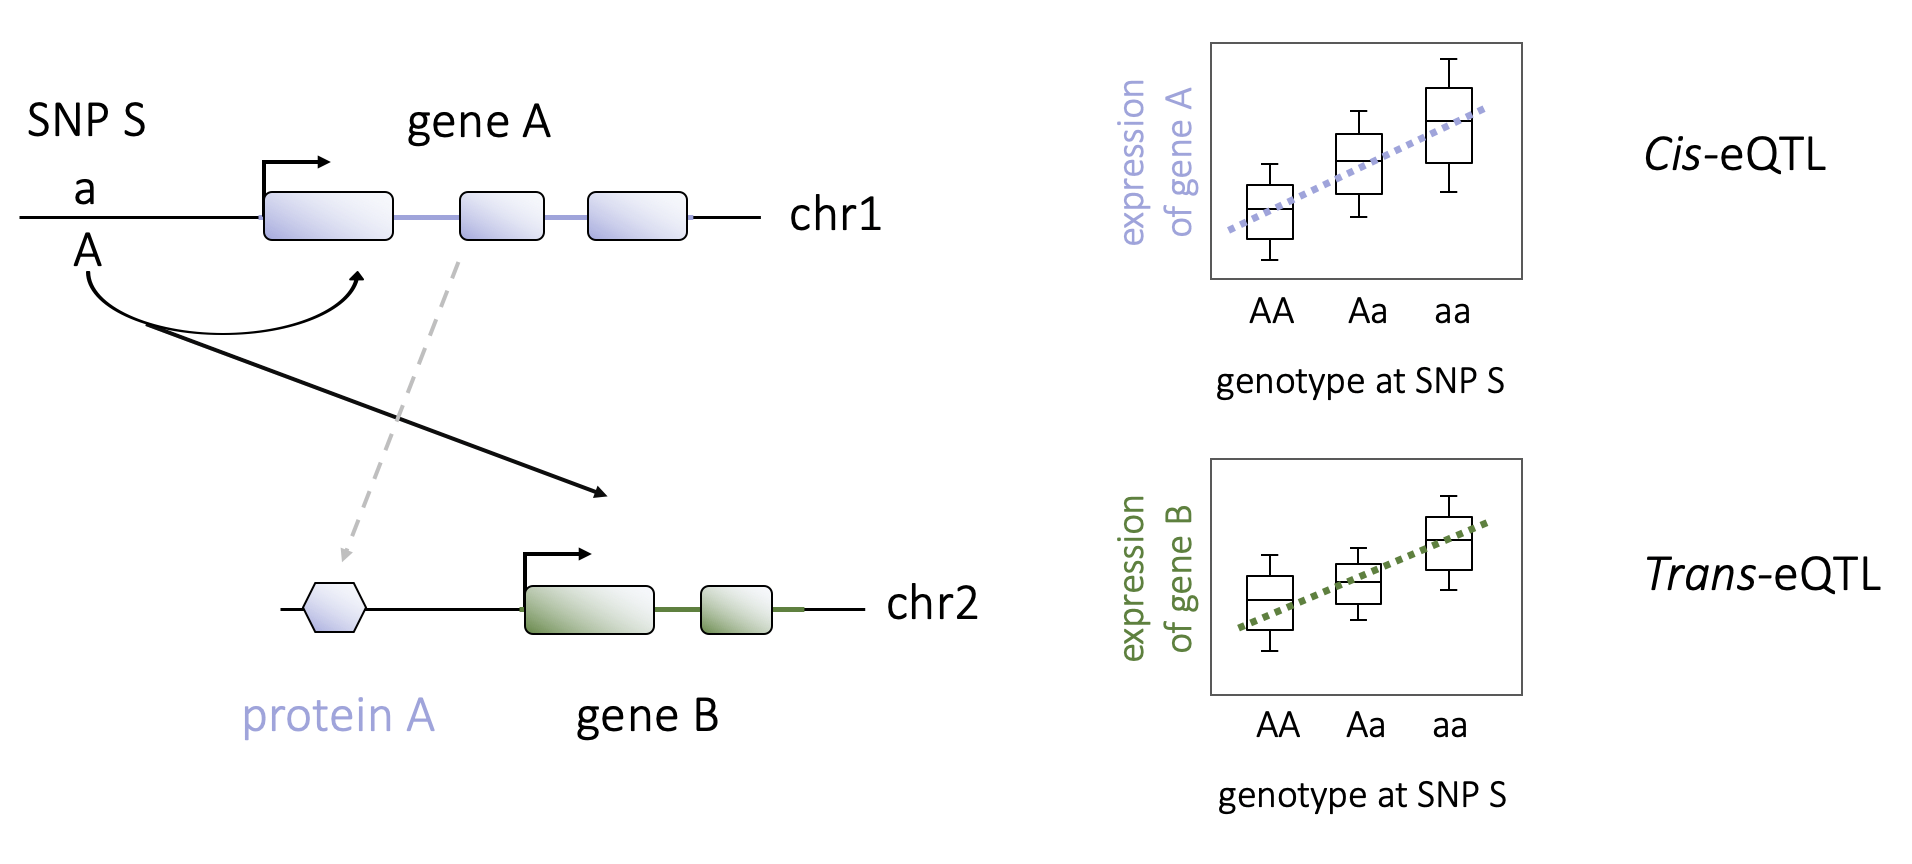
\includegraphics[width=15cm]{Chapter1/Fig/eqtl.png}
\caption[\textit{Cis} and \textit{trans} eQTL]{\textbf{\textit{Cis} and \textit{trans} eQTL}.\\
\textit{Cis} eQTL affect the expression of genes directly. 
\textit{Trans} eQTL, in contrast, affect the expression of typically more distant genes, often by first having a \textit{cis} effect on the expression of intermediate regulatory genes.
% On the right, the typical representation of eQTL using boxplots.
Figure adapted from \cite{westra2014genome}.
}
\label{fig:eqtl}
\end{figure}

% \newpage

% Variants located in the proximity  (e.g. within 1 megabase) of the affected genes are called local or proximal (putatively \textit{cis}-acting) eQTL (Fig. \ref{fig:eqtl}). 
% These variants may directly affect gene expression, or alter transcription factor binding sites or other \textit{cis}-regulatory elements (CREs), which in turn may affect transcription. 
% Indeed, it has been shown that \textit{cis} eQTL are enriched in CREs \cite{lappalainen2013transcriptome, battle2014characterizing} such as \gls{tf} binding sites and promoter regions \cite{gaffney2012dissecting}, enhancers, histone marks of active promoters and enhancers and DNase-I hypersensitivity sites \cite{degner2012dnase} and in turn tend to be depleted for repressive CREs (such as CTCF binding sites) \cite{reinhart200021, westra2014genome}. \\

% Variants affecting gene expression in a distal manner (with the variant being located more than 5Mb away from the gene or on a different chromosome entirely), usually with the help of other intermediate molecules, are called distal or (putatively) \textit{trans}-acting eQTL (Fig. \ref{fig:eqtl}, \cite{westra2014genome}).\\

Typically, \textit{cis}-eQTL have a large effect size \cite{sherman2009systematic}, thus relatively modest sample sizes (from 80-100 samples) permit the detection of \textit{cis}-eQTL for thousands of genes \cite{stranger2007population, myers2007survey}
% [17], [18], [19], [20] from \cite{westra2014genome}
. 
\textit{cis}-eQTL effects appear to be mostly additive \cite{powell2013congruence}, and \textit{cis}-eQTL SNPs are often located close to the \gls{tss} of genes or within gene bodies 
% [22], [23], [24] from \cite{westra2014genome}
\cite{vosa2018unraveling}. 
As the distance between the eQTL SNP and the \gls{tss} decreases, the eQTL effect size generally increases.
In contrast, the effect sizes of \textit{trans}-eQTL are generally small \cite{cookson2009mapping, grundberg2012mapping}. 
This, combined with the more severe multiple testing burden (see \textbf{Chapter 
\ref{chapter2}})
% 2}
mean that much larger sample sizes are required to detect \textit{trans} eQTL.
As a result, the number of reported \textit{trans}-eQTL has remained small
% [17], [19], [35], [36], [37] from \cite{westra2014genome}
\cite{grundberg2012mapping}
in comparison to the number of reported \textit{cis}-eQTL \cite{westra2014genome}.\\

In this thesis, I worked on datasets with relatively small sample sizes and only performed proximal (\textit{cis}) eQTL mapping.

% \subsubsection{eQTL are context-specific}
\subsubsection{From tissue-specific to cell type-specific eQTL}
\label{sec:eqtl_celltype_specific}

Early studies mainly performed eQTL mapping in whole blood or blood-derived cells, due to sample accessibility \cite{stranger2007population, pickrell2010understanding}.
% add some of these references from \cite{westra2014genome} below
% As such, eQTL mapping studies have now been performed in various cell-types and tissues, such as fibroblasts, 
% skin [43], 
% various purified blood cell types (e.g. lymphoblastoid cell-lines (LCLs) [43], [45],), and whole blood [19], [20], [46]).  
However, more recently, several studies have published eQTL derived from a number of normal human tissues \cite{myers2007survey, zhong2010liver,fu2012unraveling, nica2011architecture, dimas2009common, fairfax2012genetics, stranger2012patterns, schadt2008mapping, hao2012lung, innocenti2011identification}, motivated by the observation that gene expression levels vary considerably between different tissues and cell types \cite{su2002large}.
% and thus so may genetic effects on gene expression.
Perhaps most notable are those from the \gls{gtex} project, which set out to collect and analyse gene expression profiles across several primary tissues collected from post-mortem donors \cite{lonsdale2013genotype}.
Since the publication of their pilot study in 2015 \cite{gtex2015genotype}, several versions have been published \cite{gtex2017genetic, aguet2019gtex}.
The most recent version (v8) was released in 2019 and it includes data from 53 tissue types\footnote{Adipose - Subcutaneous, Adipose - Visceral (Omentum), Adrenal Gland, Artery - Aorta, Artery - Coronary, Artery - Tibial, 
Brain - Amygdala, Brain - Anterior cingulate cortex (BA24), Brain - Caudate (basal ganglia), Brain - Cerebellar Hemisphere, Brain - Cerebellum, Brain - Cortex, Brain - Frontal Cortex (BA9), Brain - Hippocampus, Brain - Hypothalamus, Brain - Nucleus accumbens (basal ganglia), Brain - Putamen (basal ganglia), Brain - Spinal cord (cervical c-1), Brain - Substantia Nigra, 
Breast - Mammary Tissue, Cells - Cultured fibroblasts, Cells - EBV-transfortmed lymphocytes,  Cervix - Ectocervix, Cervix - Endocervix, Colon - Sigmoid, Colon - Transverse, Esophagus - Gastroesophageal Junction, Esophagus - Mucosa, Esophagus - Muscularis, Fallopian Tube, Heart - Atrial Appendage, Heart - Left Ventricle, Kidney - Cortex, Kidney - Medulla, Liver, Lung,  Minor Salivary Gland, Muscle - Skeletal, Nerve - Tibial, Ovary, Pancreas, Pituitary, Prostate, Skin - Not Sun Exposed (Suprapubic), Skin - Sun Exposed (Lower leg), Small Intestine - Terminal Ileum, Spleen, Stomach, Testis, Thyroid, Uterus, Vagina and Whole Blood.} from 948 donors.
These studies have collectively identified \textit{cis} eQTL for the vast majority of human genes,
% (and increasingly for other RNA traits, splicing, transcripts, etc..),
emphasising their complex and cell type–specific nature, finding that 29\%–80\% of eQTL are cell type-specific \cite{gtex2015genotype, nica2011architecture, dimas2009common,  fairfax2012genetics}. \\

% modify highlighting importance of cell 
While eQTL from normal tissues provide valuable insights, tissues are constituted of multiple distinct cell types, each with specific gene regulatory profiles, as exemplified by the seminal work by Fairfax \textit{et al}., mapping eQTL in different blood-isolated cell types (Monocytes and B cells \cite{fairfax2012genetics}).
% \footnote{In this seminal paper, Fairfax \textit{et al} show examples cell type-sepcific eQTL in blood, e.g. variants detected as significantly affecting gene expression in monocytes, but not B cells \cite{fairfax2012genetics}}. 
% Moreover, the collection and sampling process of tissue samples from organs does not allow precise control over cell representation, adding a major source of biological variability in addition to other technical variation (McCall et al. 2016). 
Yet, except for a few studies using purified cell types \cite{fairfax2012genetics, kasela2017pathogenic, naranbhai2015genomic} or deconvolution methods \cite{westra2015cell, venet2001separation},
% including for immune cells \cite{kim2017genetic}, 
% % induced Pluripotent Stem Cells \cite{kilpinen2017common},
% and smooth muscle cells \cite{liu2018genetic}, 
eQTL datasets representing single primary cell types
% , and direct comparison of these to the tissue type of origin, 
have been lacking \cite{zhang2018cell}.
Additionally, these methods are 
% biased towards specific cell types, or are 
of limited use for less abundant cell types, and are dependent on accurately defined marker genes \cite{zhernakova2017identification}. \\
 
With the advent of single cell RNA-sequencing, eQTL mapping studies are now possible at the level of individual cells. 
scRNA-seq can be used to investigate rare cell types \cite{villani2017single}, and thus, enables identification of cell type-specific eQTL in an unbiased manner. 
A first proof-of-concept study was published in 2013 on 15 individuals, where 92 genes were studied in 1,440 cells \cite{wills2013single}.
% They observed that many eQTL are only detectable when studying single cell, and these would have been missed when the expression is averaged over multiple cells. 
In 2018, the first genome-wide single cell eQTL mapping was performed in blood, on 45 individuals \cite{van2018single}.
For further discussion on performing eQTL using single cell RNA-seq as opposed to bulk RNA-seq, see \textbf{Chapter 
% 3
\ref{chapter3}}.

\subsubsection{Context-specific eQTL}
% \subsubsection{Response eQTL}

In addition to cell type-specific eQTL,
% This is particularly interesting, because it will permit the identification of eQTL that could well depend on the specific context in which a cell operates \cite{westra2014genome}. 
% Additionally, 
some effects of genetic variants on gene expression levels have been shown to manifest themselves only within cells that have been activated by a certain external stimulus (often called response eQTL \cite{fairfax2014innate, barreiro2012deciphering, kim2017genetic}) or only in cells under certain conditions \cite{yao2014sex} - both are sometimes referred to as `context-specific eQTL' \cite{westra2014genome}. 
% If disease-associated SNPs only work in such a context, it could well be that such effects are not detectable when studying cells in bulk. 

% from Nils Kolling's thesis
% dynamic aspect
% Gene regulation differs between tissues, environments, developmental stages and cell types (The GTEx Consortium, 2013).
% For example, a SNP that causes a change to a cis regulatory module (CRM) may be identified as an eQTL in a study of liver cells. 
% However, if the transcriptional regulator that binds to this CRM is only expressed in the liver, the SNP will have no effect in another tissue. 
% A similar scenario could be imagined for different environments or developmental stages, where an eQTL found in a given environment or a given developmental stage may not necessarily have any effect in another.
% Thus, a particular focus of eQTL studies has been the identification of eQTL
% specific to various conditions, such as cell types (Dimas et al., 2009), tissues (Nica et al., 2011), temperature (Li et al., 2006) and differentiation state (Gerrits et al., 2009). 
% The relationship between eQTL and the developmental stage of a whole organism has only been investigated in one study so far (Francesconi and Lehner,
% 2014). 
% Comparing the gene expression profiles of 200 recombinant inbred lines of Caenorhabditis elegans, Francesconi and Lehner tested the association of genetic markers with the expression levels of 15,855 genes. By including the estimated developmental time point of each sample as a covariate in their test, they were able to increase the number of proximal eQTL that they could identify by 54\%.
% This led them to conclude that the developmental stage is an important factor in gene expression dynamics and the mapping of eQTL. However, the samples used in this study were not staged, which meant that developmental time point of each sample had to be estimated from its gene expression profile. 
% In addition, the mapping resolution of the study was quite limited, since it was performed on individuals from recombinant inbred lines instead of a wild population.\\

\newpage

\subsubsection{Using eQTL to link genes to disease}

Whilst useful in their own right to understand genetic regulation of gene expression across cell types and states, eQTL mapping can also be used for annotating variants associated with complex traits, as such variants are likely enriched for eQTL \cite{nicolae2010trait}. 
A recent study suggested that two-thirds of candidate common trait susceptibility genes identified as eQTL are not the nearest genes to the GWAS lead SNPs, highlighting the utility of this approach in annotating GWAS loci \cite{zhu2016integration}. 
Importantly, GWAS variants are enriched in eQTL in a tissue-specific manner. 
For instance, whole blood eQTL are enriched with autoimmune disorder-associated SNPs but not with GWAS SNPs for bipolar disorder, or type 2 diabetes \cite{gtex2015genotype}. 
These findings highlight the importance of using eQTL data from relevant cell types when following up GWAS loci for a specific disease.\\

\textbf{GWAS-eQTL colocalisation}

Integrating eQTL maps with GWAS can identify potential molecular mechanisms underlying disease associations.
One such integration method consists in testing for `colocalisation' of a GWAS trait and a gene’s expression trait - i.e. test for whether the same variant is causal to both traits \cite{cannon2018deciphering}.
Intuitively, if it can be established that a causal variant for a GWAS trait and one for a gene’s expression are the same, this may suggest a regulatory role of the causal SNP on gene expression in the pathway to the GWAS trait \cite{he2013sherlock, ongen2017estimating}. \\

However, simple overlap of GWAS and eQTL signals does not guarantee mechanism. 
First, the two variants may be two independent causal SNPs in LD with each other.
Second, eQTL are abundant \cite{lappalainen2013transcriptome}, with 48\% of common genetic variants estimated to act as eQTL for at least one gene \cite{liu2019abundant}, making the overlap between GWAS and eQTL signals possible by chance.
This motivated the development of formal statistical tests that estimate the probability of the overlaps between the two signals being due to chance - these are called colocalisation tests. \\

Early models \cite{plagnol2009statistical, wallace2012statistical, nica2010candidate} required full individual-level genotype data, which are seldom available \cite{cano2020gwas}.
% , and did not formally compare the odds of colocalisation versus a null hypothesis (Wallace, 2013), resulting in a large proportion of false positives \cite{cano2020gwas}.
More recently, Giambartolomei \textit{et al}. proposed a  colocalisation test (COLOC) which computes the odds of colocalisation compared to the null hypothesis using GWAS summary statistics \cite{giambartolomei2014bayesian}. 
Briefly, COLOC is a Bayesian statistical methodology that tests pairwise colocalisation of SNPs in GWAS with eQTL and generates posterior probabilities for each locus weighting the evidence for competing hypotheses of either no colocalisation or sharing of a distinct SNP at each locus \cite{guo2015integration}.
Since its release, COLOC has become a reference method for colocalisation testing. 
Alternative models for colocalisation include 
MOLOC (an expansion of COLOC to include multiple traits \cite{giambartolomei2018bayesian}).
JLIM \cite{chun2017limited}, 
HEIDI \cite{zhu2016integration}, 
Sherlock \cite{he2013sherlock},
% One method that accounts for multiple causal SNPs per locus is 
eCAVIAR \cite{hormozdiari2016colocalization} 
and, most recently, `jointsum' \cite{deng2020powerful}.\\

% colocalisation can also be combined with SNP-enrichment, as demonstrated by the statistical method ENLOC (Wen et al., 2017). 



\textbf{TWAS}

% In addition to providing functional insights for known GWAS loci, eQTL data may be useful for identification of novel trait-associated loci via imputation of genotype-correlated gene expression levels into GWAS datasets \cite{gamazon2015gene, gusev2016integrative}. 
% Such approaches, usually referred to as transcriptome-wide association studies (TWAS), enable assignments of potentially disease-associated loci via estimations of their genetically regulated expression.

% from \cite{cano2020gwas}
Colocalisation analyses effectively use genome-wide significant SNPs to nominate causal genes for complex traits. 
However, the majority of variants contributing to complex traits and diseases have not yet been identified, arguably because their effect sizes are too small to be detected at current GWAS sample sizes \cite{visscher201710}.
Theoretically, one may want to 
% Given that the number of genes is substantially lower than the number of common variants, using 
use tissue-specific gene expression, rather than genotypes, for association testing.
% benefits from a reduced multiple testing burden. 
However, carrying out such studies is currently unfeasible, as it would require profiling gene expression across hundreds of thousands of individuals in both cases and controls, and across dozens of tissues \cite{cano2020gwas}.
% Alternatively, (cell type-specific) gene expression profiles can be predicted (i.e. imputed) from genotypes, thus obviating the need to perform costly RNA-sequencing experiments. 
Instead,
transcriptome-wide association studies (TWAS) leverage eQTL information to predict (impute) the gene expression of the cases and controls from a GWAS, and then perform direct association of traits and genes - without directly profiling gene expression in every individual included in the GWAS \cite{wainberg2019opportunities}.
% Another way to gain insights into the biology of complex traits is by directly testing for association between a trait and gene expression (i.e., identifying which genes are expressed at a significantly different level in cases compared to controls in disease-relevant cell types). 
Several methods have been proposed, such as TWAS \cite{gusev2016integrative}, PrediXcan \cite{gamazon2015gene} and summary statistics-based Mendelian randomisation (SMR) \cite{zhu2016integration}.
% and some related methods [9,10], have been proposed recently to detect association between (the genetically regulated component of) a gene’s expression (or another molecular trait) and a GWAS trait. 
\\



% from \cite{cano2020gwas}
%  

% Predicting expression of a gene based on genotypes is possible because gene expression is highly heritable (Wright et al., 2014) and most of the gene expression heritability is attributable to variants in proximity (in \textit{cis}) to the genes (Lloyd-Jones et al., 2017). 
% TWAS uses tissue-specific eQTL maps as reference datasets to train predictors that take an individual’s genotype as an input and estimate their transcriptome levels (Gamazon et al., 2015; Gusev et al., 2016). 
% These predictors use only information from SNPs in \textit{cis} to the genes and are restricted to genes with highly heritable expression. 
% This prediction process is analogous to genotype imputation and allows for direct association between a trait and the expression of each gene (Figure 4B). Moreover, by focusing on the heritable component of gene expression, it minimises the confounding by disease-caused changes in gene expression.

% PrediXcan (Gamazon et al., 2015), an implementation of TWAS, uses an elastic net model to predict gene expression from eQTL catalogs. The authors applied this approach to data from the Wellcome Trust Case Control Consortium (WTCCC) (Wellcome Trust Case Control Consortium, 2007) and identified 41 genes associated with five complex diseases. The majority of these genes were known candidates from GWAS, while others (e.g., KCNN4 and PTPRE) had not been implicated in the diseases before. Importantly, because TWAS directly associates traits to genes, the associations have a clear directionality of effects. As an illustration, a SNP nearby ERBB3 had been previously associated with type 1 diabetes (Hakonarson et al., 2008). PrediXcan confirmed the association between ERBB3 and type 1 diabetes and found that low ERBB3 expression increased disease risk (Gamazon et al., 2015). Defining the directionality of effects of GWAS variants, and particularly identifying risk variants which increase gene expression, can nominate effective drug targets and accelerate the development of new therapies.

% To overcome the requirement for individual-level genotypes, the authors of PrediXcan subsequently derived a mathematical formulation (S-PrediXcan) which achieves comparable results using GWAS summary statistics (Barbeira et al., 2018). The authors applied S-PrediXcan to over 100 phenotypes across 44 GTEx tissues and found that most of the associations detected were tissue-specific, highlighting the need to profile gene expression in disease-relevant cell types. For example, LDL levels were positively associated with SORT1 expression only in the liver and negatively associated with PCSK9 only in tibial nerve. In contrast, schizophrenia was negatively associated with C4A expression across 42 of the 44 tissues tested (Barbeira et al., 2018).

% Because most of the SNPs used to predict gene expression in TWAS are enriched in regulatory DNA (Trynka and Raychaudhuri, 2013), including epigenetic annotations in the model can improve transcriptome imputation. EpiXcan is an implementation of PrediXcan which takes into account annotations such as DNA methylation or histone modifications (Zhang et al., 2019). The contribution of each SNP in the prediction is weighted by its overlap with regulatory elements in a Bayesian hierarchical model. When applied to 58 traits and 14 eQTL datasets, EpiXcan increased the number of gene-trait associations by over 18% compared to PrediXcan. Most of these associations were tissue-specific. For example, TWAS associations with CAD were only detected in arterial tissue, while schizophrenia associations were specific to the brain (Zhang et al., 2019). Moreover, integrating EpiXcan with a catalog of chemical perturbations revealed drug repurposing opportunities. An example is ursolic acid, which can reverse the gene expression changes associated with BMI. This compound is currently under investigation for the treatment of obesity (Kunkel et al., 2012).

% Another TWAS approach proposed by Gusev et al. (2016) uses a Bayesian predictor to impute gene expression from genotypes. First, the method determines the weights of the Bayesian predictor based on a reference eQTL catalog. The contributions of each variant to the predictions are proportional to its eQTL effects on each gene. Next, gene expression is imputed directly from the GWAS summary statistics. To do this, the authors first use the summary statistics to impute the GWAS effect sizes of all common variants (Pasaniuc et al., 2014) and then multiply these effect sizes by the Bayesian weight of each variant (determined from the eQTL catalog as previously described). Each variant is then re-weighed by its LD with other variants in the locus. Finally, the contribution of all variants proximal to a gene is combined into a single expression-trait association estimate. The authors used this approach to find genes involved in the regulation of circulating lipid levels (HDL, LDL, total cholesterol, and triglycerides). This analysis nominated 665 lipid-associated genes, of which 66 had not been previously identified by any of the independent GWAS (Gusev et al., 2016). The majority of these novel genes showed additional functional evidence from mouse studies. For example, FTSJ3 expression correlated with fat mass and glucose-to-insulin ratio in mice, while ITIH4 correlated with LDL levels.

% Gusev et al. (2018) subsequently extended their approach to epigenetic data. The authors performed a TWAS to test for association between gene expression in brain tissue and risk for schizophrenia, including as an additional layer of information chromatin marks (i.e., H3K27ac, H3K4me1, and H3K4me3) assayed in 76 lymphoblastoid cell lines. This allowed them to nominate both genes and regulatory elements involved in disease. For example, the authors found two chromatin elements associated with MAPK3 expression, which was in turn associated with schizophrenia risk. They then functionally validated this association, showing that MAPK3 is involved in a neuro-proliferation phenotype in zebrafish (Gusev et al., 2018).

% Finally, summary data-based Mendelian randomisation (SMR) uses a Mendelian randomisation (MR) framework to perform a TWAS analysis (Zhu et al., 2016). MR takes advantage of the fact that an individual’s genotype is independent of confounding factors such as nurture or environmental covariates. In traditional MR, genotypes are used as an instrumental variable to infer causal relationships between an exposure (e.g., the levels of a metabolite or protein) and a trait (e.g., a disease) (Evans and Davey Smith, 2015). In SMR, an analogous approach is used to infer associations between gene expression and a trait. In brief, the authors use genetic variants as instrumental variables and estimate the effect size of a gene in a trait as the ratio of the GWAS effect size to the eQTL effect size of a variant affecting the expression of the gene (Zhu et al., 2016). Traditional TWAS approaches impute gene expression from genotypes and then associate genes to traits. However, because imputation is based on the combined effects of multiple proximal variants, TWAS cannot directly point to the individual variants underlying gene-trait associations. In contrast, SMR estimates a separate gene-trait effect size from each individual SNP in a locus, thus making it possible to link variants to genes. By comparing the effect-sizes derived from all the SNPs in a locus, SMR is able to identify cases in which a single variant affects both gene expression and a complex trait. This test (HEIDI) is a form of colocalisation analysis (Zhu et al., 2016). However, since most gene-trait effects are small due to polygenicity (Boyle et al., 2017), SMR requires eQTL catalogs of very large sample size. The authors applied SMR to a large peripheral blood eQTL study (5,311 samples) (Westra et al., 2013) and identified 289 genes associated with body-mass index, waist-hip ratio, rheumatoid arthritis and schizophrenia. Of these, 104 genes showed evidence of a single causal variant. An interesting example includes a locus associated with rheumatoid arthritis which contains the genes TRAF1 and C5. Based on its function, TRAF1 had been prioritised as the most likely target gene. SMR confirmed the prioritisation of TRAF1 and provided evidence of a single causal variant in the region (Zhu et al., 2016).

In summary, colocalisation and TWAS both combine eQTL and GWAS catalogues with the aim to prioritise the genes causally involved in complex diseases.
Colocalisation analysis integrates association signals from GWAS and eQTL on a locus by locus basis to identify instances in which both traits share a causal variant. 
In contrast, TWAS leverages information from eQTL catalogs to impute gene expression values and directly associate genes to traits. 
The availability of eQTL catalogs from a wider variety of cell types, as well as of larger sample sizes, will improve gene prioritisation and translate GWAS results to refined sets of disease-causal genes \cite{cano2020gwas}.



% Transcriptome-wide association analysis (TWAS) on the other hand, aim to identify associations between gene expression and traits and diseases 
% \cite{mancuso2018large, wainberg2019opportunities}.

% papers from Bogdan Pasaniuc
% Wainberg et al - review (2019) \cite{wainberg2019opportunities}

\subsubsection{eQTL mapping in iPSC and iPSC-derived cells}

In addition to human primary tissues, \glspl{eqtl} have been described in human \glspl{ipsc} and \gls{ipsc}-derived cells (see \textbf{section \ref{sec:ips_genetics}}).
In the second part of this introduction (\textbf{section \ref{sec:human_ipscs}}), I describe the use of \glspl{ipsc} as an \textit{in vitro} model for early human development and as a resource to generate donor-matched cell types and tissues that are impossible to access \textit{in vivo}.
Population-scale \gls{ipsc} derivation and differentiation provides an outstanding resource to investigate the role of genetic variants on expression in disease-relevant tissues and during development.
% Additionally, iPSC allow manipulation and stimulation..


% ***********************************************************************************************************************************************************************************************************************************************************************************************************************************

\newpage

\vspace*{10px}

\textit{“It is not birth, marriage, or death, but gastrulation which is truly the most important time in your life.”}\\
\rightline{Lewis Wolpert, 1986}

\vspace*{5px}

% ***************************************************************
%************************ %Second Section %****************************************************************

\section{Human iPSCs to study cell differentiation}  %Section - 1.2
\label{sec:human_ipscs}  

Human \glspl{ipsc} and cells derived therefrom are the biological system I use throughout this thesis to study the effect of common genetic variants on expression during cell differentiation.
I use this section to provide some basics of human embryology and to describe the role of human stem cells in scientific research.
I focus especially on the \gls{ipsc} technology, which allows reprogramming of cells from easily accessible somatic tissues such as skin and blood to regain stem-cell like (pluripotent) properties and to be subsequently differentiated into virtually any desired cell type, provided the right stimuli.\\

In particular, in \textbf{section \ref{sec:history_developmental_biology}}, I provide a brief historical overview of the study of early development in humans and in \textbf{section \ref{sec:human_embryogenesis}} I describe the key stages of human embryology, which we attempt to mimic using \gls{ipsc}-derived differentiation protocols.
Then, in \textbf{sections \ref{sec:escs}} and \textbf{\ref{sec:cloning}}, I introduce the two key concepts of \glspl{esc} and \gls{scnt}, or somatic cloning.
\glspl{esc} are cells collected at a very early stage of the embryo's development that can be grown \textit{in vitro} to model development.
Somatic cloning, on the other hand, involves introducing the nucleus of a donor's somatic cell into an enucleated ovum which can either be implanted into a host and let develop, creating a `clone' for the donor; or, alternatively, grown \textit{in vitro} for research purposes.
 
Next, in \textbf{section \ref{sec:ipsc}}, I describe induced pluripotent stem cells, a technology that allows somatic cells to be reprogrammed to a pluripotent state, which can, in turn, be differentiated into virtually any
% \footnote{Excluding extra-embryonic cells \cite{}.} 
somatic cell types.
This allows the generation of \gls{esc}-like cells directly from a(ny) donor, bypassing the need for cloning. 
In this section I will describe the technology and highlight advantages and challenges of the use of \glspl{ipsc} in biological research.
Finally, in the last section (\textbf{section \ref{sec:ips_genetics}}), I describe 
applications of human \glspl{ipsc} generated from many individuals to perform population-scale genetic analyses across a variety of \gls{ipsc}-derived cell types.
% general applications of human stem cells in biology, focusing in particular on applications of \glspl{ipsc} for human genetics.

% %********************************** % 1.2.1  **************************************
\newpage

\subsection{From homunculi to developmental biology}
\label{sec:history_developmental_biology}

In the previous section, we learnt that DNA encodes all instructions of life, and that each one of us contains a mixture of genetic information from both parents, which is identically copied in every one of our cells.
But how do we go from one single cell containing our genetic fingerprint to a whole organism made of some 37 trillion highly specialised cells which differ in function and morphology and work together in harmony as a single organism?\\

Interest in the study of human development and the embryo has ancient origin.
We define an embryo as the first stages of development of a fertilised ovum in the uterus.
The word derives from the Greek \textepsilon\textmu\textbeta\textrho\textupsilon\textomikron\textnu \ (embryon, literally `young one').
Early embryology (from embryon and -\textlambda\textomikron\textgamma\textiota\textalpha, -logia, `study of') was first proposed by an Italian, Marcello Malpighi, and was intended as preformationism.
The theory of preformation believes that an embryo is contained in the semen (thus only derives from the father) and that it is essentially a preformed miniature infant (`homunculus') which just gets larger and larger during development (\textbf{Fig. \ref{fig:early_embryology}}).\\

\begin{wrapfigure}{r}{0.6\textwidth}
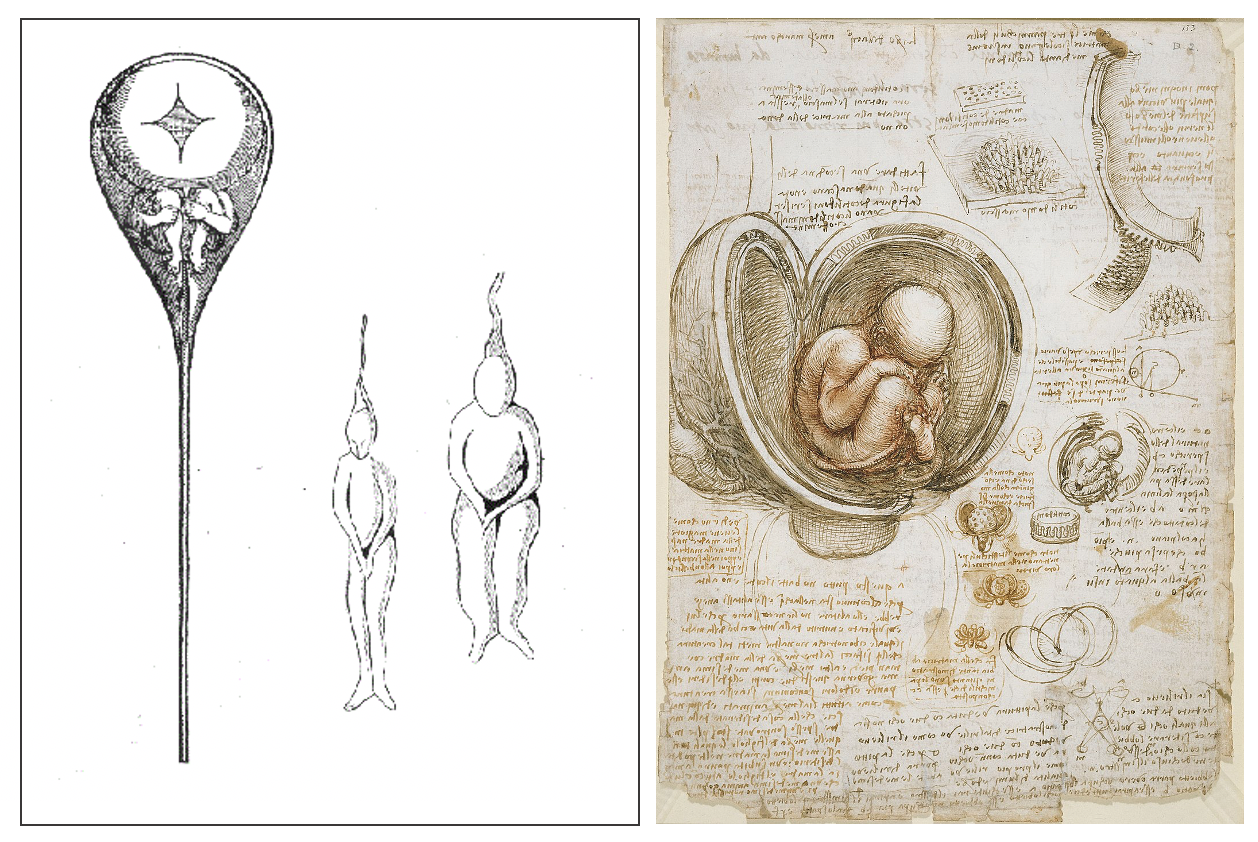
\includegraphics[width=9.5cm]{Chapter1/Fig/Early_theories_development.png}
\caption[Early theories of development]{\textbf{Early theories of development}.\\
Illustration of the two leading theories on human embryology before the 19$^{th}$ century.
Left, Illustration of Preformation: 
A tiny person (homunculus) growing inside a sperm, as drawn by Nicolaas Hartsoeker in 1695.
Right, Epigenesis: study of foetus deveopment by Leonardo Da Vinci, c. 1510.}
\label{fig:early_embryology}
\end{wrapfigure}

The competing explanation of embryonic development was epigenesis, originally proposed 2,000 years earlier by Aristotle. 
Much early embryology and support for the epigenesis theory came from the work of Italian anatomists such as Aldrovandi and Leonardo da Vinci (\textbf{Fig. \ref{fig:early_embryology}}) in the Renaissance.
According to epigenesis, the form of an animal emerges gradually from a relatively formless egg. 
Yet for centuries, most people believed in preformationism over epigenesis.
Only as microscopy improved during the 19th century, could biologists see that embryos took shape in a series of progressive steps, and epigenesis displaced preformation as the favoured explanation among embryologists.\\

Modern embryology developed from the work of Estonian-born Karl Ernst von Baer.
Von Baer is credited with discovering the mammalian ovum in 1827 and became the first person to observe human ova.
Only in 1876 did Oscar Hertwig prove that fertilisation is due to the fusion of an egg and a sperm cell \cite{hertwig1875beitraege}.
Additionally, von Baer laid the foundation for the field of comparative embryogenesis in his `On the developmental history of animals', published in 1828 \cite{von1828entwickelungsgeschichte}.
In it, he formulated what became known as Baer's law of embryology.
In particular, he observed that large changes in embryo development precede more specific changes and that at a time in development embryos from different species look very similar, despite looking very different as adults.
Some of his ideas were later used by Darwin in his theory of evolution.
In his study of embryology, Von Baer discovered the blastula and formulated the germ layer theory.\\

Human embryology as a scientific discipline is linked to the creation of human embryo collections \cite{yamada2015human, gasser2014rebirth, shahbazi2020mechanisms}. 
The pioneering work of Franklin Mall led to the creation of the Carnegie collection in 1887, which harbours more than 10,000 human embryo specimens, and established the basic staging criteria for the developmental classification of human embryos \cite{keibel1910manual}. 
Other collections were later created, such as the Kyoto collection, which today holds around 44,000 specimens \cite{nishimura1968normal}. 
Much of our current textbook knowledge of human development is derived from the early descriptive studies of these samples.\\

% rewrite and add references 
The development of \textit{in vitro} fertilisation (IVF) of human eggs \cite{edwards1969early, rock1944vitro, shettles1955morula}, followed by the development of conditions to culture these fertilised eggs for up to 5-6 days \cite{edwards1970fertilization, steptoe1971human},
% , and ultimately led to the birth of the first IVF baby in 1978, thanks to the tireless efforts of Robert Edwards, Patrick Steptoe and Jean Purdy.
% Since then, the field of human embryology has flourished. 
% IVF has 
allowed scientists to describe the dynamics of key morphogenetic processes during early human development (see \textbf{section \ref{sec:human_embryogenesis}}).
% , such as cleavage, compaction and blastulation (Wong et al., 2010; Marcos et al., 2015; Iwata et al., 2014); to characterise cell lineage specification events by studying the transcriptional and epigenetic profiles of all the cells present in a developing human embryo (Niakan and Eggan, 2013; Petropoulos et al., 2016; Braude et al., 1988; Zhu et al., 2018); to identify genetic and chromosomal abnormalities that compromise human embryo development (Munne et al., 2009; Vanneste et al., 2009); and, perhaps more importantly, to establish human embryonic stem cell lines \cite{thomson1998embryonic}, which on their own have revolutionised our approach to studying human development and devising regenerative therapies. However, until recently, gene function could not be studied in the context of human embryos. 
% The recent generation of OCT4 knockout human embryos represents a turning point in the field (Fogarty et al., 2017). 
% This study highlighted differences in gene function between mouse and humans, and established a gold standard for functional studies in human embryos.
% Thus, human embryology is becoming an experimental science; I argue that, in the years to come, we will witness a surge in the number of mechanistic studies exploring our own development \cite{shahbazi2020mechanisms}.
\\

% After the 1950s, with the helical structure of DNA being unraveled and with increasing knowledge in the field of molecular biology, developmental biology emerged as a field of study that attempts to determine which genes are responsible for morphological changes taking place in an embryo, and how these genes are regulated.

% Development requires mechanical changes in cell and tissue shape, which drive morphogenesis, and gene expression changes, which regulate cell fate decisions and tissue patterning. These two developmental processes are not independent, as changes in cell fate can modify the architecture of tissues, and vice versa (Chan et al., 2017). Mechanochemical feedback at the molecular, cellular and tissue levels coordinates this crosstalk and instructs tissue self-organisation (see Glossary, Box 1) (Hannezo and Heisenberg, 2019).

In parallel, ever since the 1950s, with the helical structure of DNA being unraveled (see \textbf{section \ref{sec:double_helix}}), and with increasing knowledge in the field of molecular biology, developmental biology had emerged and was growing rapidly as a field of study
% re-write and combine below
that attempts to determine the interplay between morphological and gene expression changes during embryogenesis.
% which genes are responsible for morphological changes taking place in an embryo, and how these genes are regulated.\\
Indeed, development requires both mechanical changes in cell and tissue shape, which drive morphogenesis, as well as gene expression changes, which regulate cell fate decisions and tissue patterning \cite{niakan2013analysis, petropoulos2016single}. 
% These two developmental processes are not independent, as changes in cell fate can modify the architecture of tissues, and vice versa (Chan et al., 2017). 
Mechano-chemical feedback at the molecular, cellular and tissue level coordinates this crosstalk and instructs tissue self-organisation \cite{hannezo2019mechanochemical}.

\newpage

\subsection{Human Embryogenesis}
\label{sec:human_embryogenesis}

% add key genes and signalling
% could take from \cite{shahbazi2020mechanisms}
% Nanog, Gata6 (endoderm), 
% Wnt signalling / TGF-beta signalling / Nodal signalling

I use this section to briefly outline the key steps of human embryogenesis as this is the system we aim to mimic \textit{in vitro} using differentiating human iPSCs.
Embryogenesis describes the first eight weeks of development\footnote{covering the 23 Carnegie stages.
The Carnegie system was based on work by Streeter \cite{streeter1942developmental} and O'Rahilly and Müller \cite{o1973developmental, o2010developmental} at the Carnegie Institution of Washington.
The system is standardised and provides a unified developmental chronology of the vertebrate embryo.} after fertilisation, after which we generally refer to fetal development \cite{gilbert2008developmental}.\\

Thanks to technological advances in microscopy and \textit{in vivo} experiments in model organisms such as fruit flies and mice, we have learnt a lot about this process since the pioneering experiments of von Baer.
In particular, embryogenesis starts with a zygote, which is the single cell resulting from the fusion of gametes, an egg and a sperm cell; the fusion is known as fertilisation.
Then, the first 12-to-24 hours post fertilisation are spent in cleavage, which consists of very rapid cell (mitotic) division and no growth.\\

Around day 3 cells start to get clumped together in a process called compaction \cite{iwata2014analysis}.
At this point (day 3/4), the 16-32 cell embryo is called the morula (which is the Greek word for mulberry), which will undergo blastulation \cite{wong2010non} (\textbf{Fig. \ref{fig:embryogenesis}}).
Around day 4, cells continue to divide, but they also begin to differentiate and develop more specific forms and functions.
Two layers develop: the cells on the outer layer are called trophoblasts, and the cells inside are embryoblasts
% in mouse, this is mediated by YAP
\cite{petropoulos2016single, niakan2013analysis}. 
Next, at around day 5, the embryoblasts clump even further into an inner collection of cells called the inner cell mass, which is pushed to a side of the sphere formed by the trophoblast.
The rest of the fluid-filled cavity is called the blastocoel and this conformation is called blastocyst.
This is also the time when the zona pellucida (a protective membrane that surrounded the egg cell and that was limiting the embryo's growth) begins to disappear, allowing the blastocyst to grow, change shape and start moving \cite{larsen2001human}.\\

The ability of the embryo to move allows the beginning of implantation: around day 7 the embryo has now left the Fallopian tube and reached the uterus and attaches to its wall, the endometrium.
The trophoblasts divide and then fuse with the endometrium -
% they are now called syncitio-trophoblasts (vs cytotrophoblasts normal) and form villi uterine blood vessels and fetal blood vessels can transfuse into each other 
% together they
initiating the process that 
will eventually build the placenta.\\

% Up to this point, cells in the inner cell mass are pluripotent, meaning that they can eventually turn into the cells of any body tissue (muscle, brain, gut, etc). 
During the second week, these cells form another cavity, called the amniotic cavity. 
At the same time, they start differentiating further into two layers: the epiblast (closer to the amnitioc cavity) and the hypoblast (closer to the blastocoel). 

\begin{figure}[h]
\centering
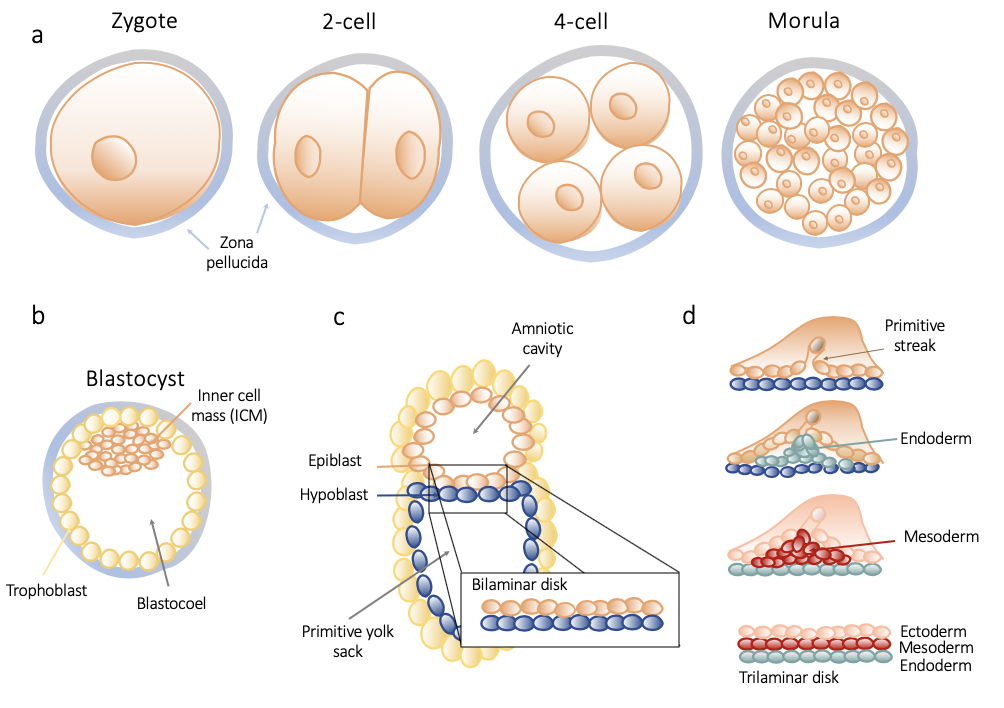
\includegraphics[width=14.5cm]{Chapter1/Fig/embryogenesis_til_gastrulation.png}
\caption[Human Embryogenesis]{\textbf{Human Embryogenesis}.\\
Early stages of human embryogenesis.
(a) From zygote to morula: stages of clevage.
(b) The blastocyst.
Cells divide and form an outer layer, the trophoblasts.
Inner cells also called embryoblasts get compacted and move to a side forming the inner cell mass (ICM), leaving a fluid filled cavity called the blastocoel.
(c) The formation of the bilaminar disk.
The ICM splits into the epiblast and hypoblast which distribute along the surface and result into two more cavities, the amniotic cavity and the primitive yolk sac, respectively.
(d) Gastrulation: from bilaminar to trilaminar disk.
The primitive streak forms and cells start to migrate moving down in between the epiblast and the hypoblast.
The endoderm, mesoderm and ectoderm form and are called the trilaminar disk.}
\label{fig:embryogenesis}
\end{figure}

Together, the epiblast and the hypoblast form the bilaminar disc \cite{hertig1956description}.
The hypoblast does not contribute to the embryo, so we will now turn our focus solely on the epiblast (\textbf{Fig. \ref{fig:embryogenesis}}).\\

The next stage of early embryogenesis is gastrulation \cite{sheng2015epiblast}.
Famously called “the most important moment in your life” by Lewis Wolpert \cite{wolpert2015interview}, gastrulation is the process during which the three germ layers (endoderm, mesoderm and ectoderm) form.
The cell mass is now known as a gastrula.
% A germ layer is a layer of cells that will go on to form one of our organisational tubes.
The first step of gastrulation is the formation of the primitive streak ($\sim$day 16).
This streak determines the midline of the body, and separates the left and right sides.
At this point, cells are moving down from the epiblast, ending up between the original epiblast layer and the hypoblast.
The first layer to invaginate dives the deepest and ends up closest to the hypoblast - this is the endoderm.
The next layer forms the mesoderm, and the remaining epiblast cells that continue to border the amniotic cavity are the ectoderm (\textbf{Fig. \ref{fig:embryogenesis}}).\\

The next stage is called neurulation (week 3-5).
Directly beneath the primitive streak the mesoderm (the middle germ layer) forms a thin rod of cells known as the notochord.
The notochord induces a change within the ectoderm above it, leading to the formation of the neural plate which then dives into the mesoderm to form the neural tube.
This is the end of what is called `early embryogenesis'.\\

Next, the germ layers start forming the various organs in a process called organogenesis.
Briefly, the endoderm forms the gastro-intestial tract, from which upper tract the lungs, the liver and the pancreas form. 
The tube itself forms the esophagus, the stomach, and the small and large intestines.
Second, the mesoderm forms some inner layers of the skin (endothelial cells), the muscles (including the heart), the bones and then also the kidneys and the bladder, ovaries and/or testis and blood cells.
Finally, the ectoderm forms the outer layer of the skin (epithelial cells), sweat glands and hair, and importantly our nervous system.
After eight weeks since fertilisation, we call the embryo a foetus, and fetal development begins.

% \subsubsection{Mechanisms of differentiation}

% Cues can be internal and external.

% Internal:

% zygote contains transcription factors (TFs) which will activate certain genes as well as their mRNA recursors.
% TFs are all clustered in one area of the zygote so as cells divide cells that were in the TF-rich region of the zygote will have many TFs while others will have barely any.
% This is known as `asymmetric segregation of cellular determinants'.

% External: induction

% One group of cells can induce another group of cells to differentiate using signalling, which can be in the form of diffusion, direct cell-to-cell contact or gap junctions (connexon proteins) between cells.

% % Examples: limbs, ears, eyes

\newpage

% %********************************** % 1.2.3 **************************************
% \subsection{Embryonic Stem Cells}
% \label{sec:escs} 

\subsection{Human Stem Cells}
\label{sec:escs} 

% look up in humans
In mammals, roughly 50–150 cells make up the inner cell mass during the blastocyst stage of embryonic development, around days 5–14 (\textbf{Fig. \ref{fig:embryogenesis}}). 
These have stem cell\footnote{stem cells are characterised by their self-renewing abilities and the `potency' to differentiate into more specialised cells.} capability, meaning that they can eventually differentiate into all of the body's cell types (making them `pluripotent').
% Inner cell mass stem cells are sometimes called `embryonic' stem (ES) cells to differentiate them from other types of stem cells found in the adult body, called somatic or adult stem cells.
% to maintain stem cell numbers:
% 1) obligate asymmetric replication i.e. each stem cell as it divides creates another stem cell and a differentiated cell
% 2) stochastic differentiation i.e. if one stem cells makes two differentiated cells instead, another will make two stem cells to balance it out
Only the zygote is considered to be truly `totipotent' as it is able to form not only cells of the body (derived from the epiblast) but extra-embryonic tissues as well (from the hypoblast), which are necessary for the formation of a living organism.
% Compared to ESCs, adult stem cells are less plastic, less potent.
Cells with stem-cell properties are still present in the adult body, and are called somatic or adult stem cells.
These are less 
% plastic (less 
potent
% ) 
than inner mass cells.
In particular, some adult stem cells have the ability to differentiate into a whole suite of cell types, and are called `multipotent'.
For example, this is the case for hematopoietic stem cells, which give rise to all the cell types of the blood and the immune system.
Other stem cells are more specialised, like epidermal stem cells, which are only able to differentiate into epidermal cells, or fibroblasts.
These are called `unipotent' (\textbf{Fig. \ref{fig:stem_cells}}).\\

\begin{figure}[htbp]
\centering
% 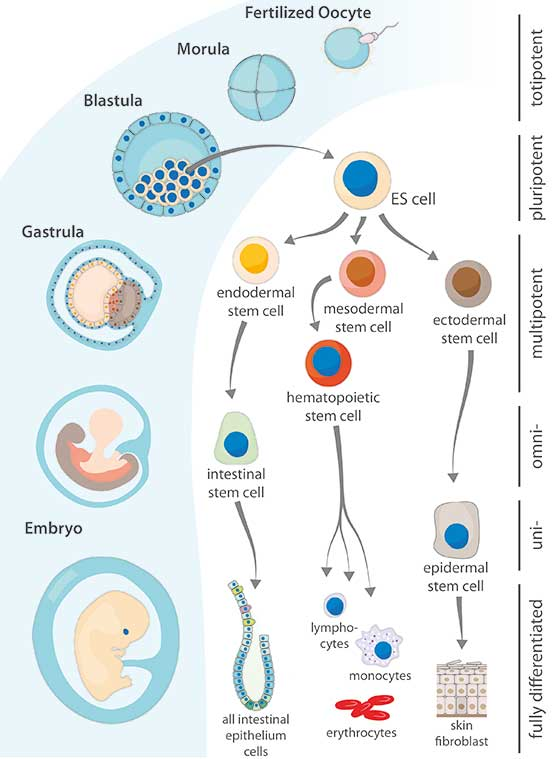
\includegraphics[width=13cm]{Chapter1/Fig/stem_cells.jpg}
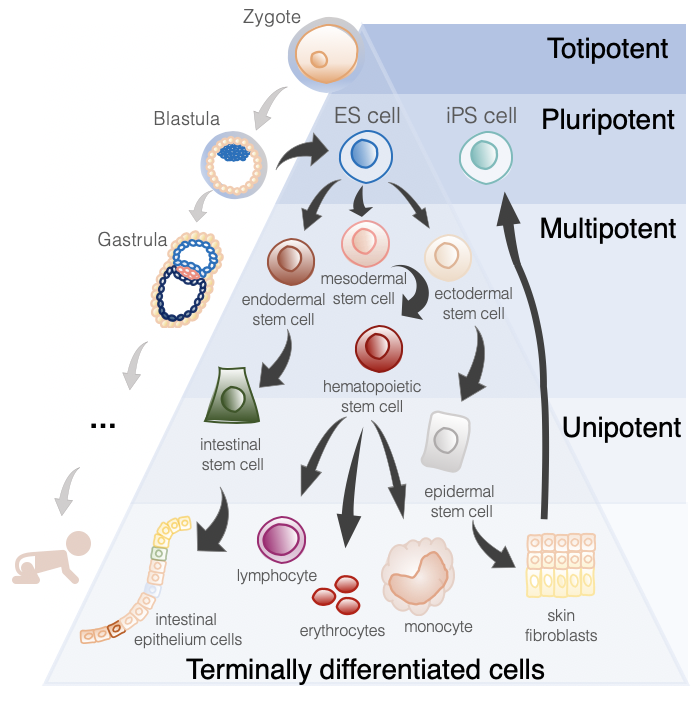
\includegraphics[width=16cm]{Chapter1/Fig/stem_cell_potency.png}
\caption[Stem Cells]{\textbf{The potency tree of stem cells}.\\
The spectrum of potency along development: from the totipotent zygote to terminally differentiated cells. 
% (from \url{https://www.enzolifesciences.com/science-center/technotes/2019/august/stem-cells-from-embryonic-origin-to-induced-pluripotency-an-overview/}).
}
\label{fig:stem_cells}
\end{figure}

The existence of stem cells was first demonstrated by Canadian biologists Ernest McCulloch and James Till in the early 1960s.
Together with graduate student Andy Becker and senior scientist Lou Siminovitch their work was published in \textit{Nature} in 1963 \cite{becker1963cytological}.

\subsubsection{Embryonic stem cells}

% As mentioned, inner mass cells are pluripotent.
% \textit{In vivo}, they go on to differentiate into the three germ layers (during gastrulation) and then make up organs (during organogenesis).
% In general, differentiation is thought to be a one-way street, meaning that more specialised cells cannot go backwards to stem cells naturally.
% Inner mass cells, when they are isolated and cultured \textit{in vitro}, can be kept in the stem-cell stage and are known as \glspl{esc}.
In 1981, \gls{es} cells were first isolated and successfully cultured using mouse blastocysts by British biologists Martin Evans and Matthew Kaufman \cite{evans1981establishment, martin1981isolation}.
In the 1990s, \gls{es} cell lines from two non-human primates, the rhesus monkey \cite{thomson1995isolation} and the common marmoset \cite{thomson1996pluripotent}, were derived, and these offered closer models for the derivation of human \gls{es} cells. 
The first \glspl{hesc} were finally isolated in 1998 by the American developmental biologist James Thomson \cite{thomson1998embryonic}.
Thomson and colleagues derived \gls{hesc} lines by culturing human blastocysts in a cocktail of growth factors and supporting mouse feeder cells.
Indeed as they first demonstrated, human inner mass cells, when isolated and cultured \textit{in vitro}, can be kept in the stem-cell stage and are known as  \glspl{hesc}. \\

% from \cite{department2006regenerative}
Because they can proliferate without limit and can contribute to any cell type, human \gls{es} cells offer unprecedented access to tissues from the human body \cite{department2006regenerative}. 
% They will support basic research on the differentiation and function of human tissues and provide material for testing that may improve the safety and efficacy of human drugs (Figure 1.3: Promise of SC Research).7,8 
% For example, new drugs are not generally tested on human heart cells because no human heart cell lines exist. 
% Instead, researchers rely on animal models. 
% Because of important species-specific differences between animal and human hearts, however, drugs that are toxic to the human heart have occasionally entered clinical trials, sometimes resulting in death. 
% Human ES cell-derived heart cells may be extremely valuable in identifying such drugs before they are used in clinical trials, thereby accelerating the drug discovery process and leading to safer and more effective treatments.9–11 
% Such testing will not be limited to heart cells, but to any type of human cell that is difficult to obtain by other sources.\\

% Human ES cells also have the potential to provide an unlimited amount of tissue for transplantation therapies to treat a wide range of degenerative diseases. 
% Some important human diseases are caused by the death or dysfunction of one or a few cell types, e.g., insulin-producing cells in diabetes or dopaminergic neurons in Parkinson's disease. 
% The replacement of these cells could offer a lifelong treatment for these disorders.
% However, there are a number of challenges to develop human ES cell-based transplantation therapies, and many years of basic research will be required before such therapies can be used to treat patients. 
% Indeed, basic research enabled by human ES cells is likely to impact human health in ways unrelated to transplantation medicine. 
% This impact is likely to begin well before the widespread use of ES cells in transplantation and ultimately could have a more profound long-term effect on human medicine. 
% Since August 2001, improvements in culture of human ES cells, coupled with recent insights into the nature of pluripotency, genetic manipulation of human ES cells, and differentiation, have expanded the possibilities for these unique cells.

% Culture of ES cells
% Mouse ES cells and human ES cells were both originally derived and grown on a layer of mouse fibroblasts (called feeder) in the presence of bovine serum.

% A feeder-free human ES cell culture system has been developed, in which human ES cells are grown on a protein matrix (mouse Matrigel or Laminin) in a bFGF-containing medium that is previously conditioned by co-culture with fibroblasts \cite{xu2001feeder}.

% The status of imprinted (epigenetically modified) genes and the stability of imprinting in various culture conditions remain completely unstudied in human ES cells**. The status of imprinted genes can clearly change with culture conditions in other cell types.28,29

%%

As a consequence, \gls{hesc} lines held great promise for research purposes, as an \textit{in vitro} model for both human development and disease \cite{saha2009technical}.
First, embryonic stem cells have been used widely to improve our understanding of embryogenesis and development in general. 
Both in human and mouse, \glspl{esc} have been differentiated into a plethora of cell types.
Additionally, \glspl{esc} can be grown not only in a 2D culture but also in 3D structures, to better mimic the formation of organs (i.e. organoids \cite{clevers2016modeling, lancaster2013cerebral}) or even entire (early) embryos (the so called `gastruloids' \cite{van2020single2}). \\

Second, exciting prospective applications included \textit{in vivo} drug testing as well as, importantly, cell replacement therapy: ever since, the use of pluripotent stem cells for regenerative medicine has been sought \cite{kimbrel2015current}.
Indeed, not only do \glspl{esc} have the ability to self-renew indefinitely, but in theory they can also be differentiated into any cell type in the body, thus providing functional replacement or trophic support to worn-out or dysfunctional cells and tissues in a range of diseases. 
% \\
% combine with above
\\

However, in order to isolate \glspl{esc} the embryo needs to be destroyed which, naturally, caused a big ethical debate.
Such ethical concerns caused the generation of \glspl{esc} to be reduced substantially or even made illegal in some countries.

Today, a number of lines have been isolated and frozen and are available for research.
Stem cell banks from a few countries provide (managed) access to several hundred \gls{hesc} lines including the UK Stem Cell Bank (139 lines) and the US NIH Human Stem Cell Registry (484 lines).
% \url{https://www.nibsc.org/ukstemcellbank} ref UK
% \url{https://grants.nih.gov/stem_cells/registry/current.htm} ref US
In total, it is estimated that there are between 800 and 1,000 \gls{hesc} lines available in the world which are, in the vast majority, derived from discarded IVF\footnote{\textit{In vitro} fertilisation.} embryos \cite{isasi2009governing}.\\
% How many? Where? All healthy?
% This of course means that these lines have been carefully scrutinised and are optimised for...

% \subsubsection{Stem Cell systems}
% Embryonic stem cells \& Organoid models



% Embryoid Bodies (EBs) - ESCs left to aggregate with the addition of some cytokines (Brickman and Serup 2016, Spangler et al 2018)

% micropatterns: MPA vs MPP (anteriorly or posteriorly biased)
% Morgani et al 2018

% Gastruloid can break symmetry - form antero-posterior axis (van de Brink et al 2014, van den Brink 2020)

% PGC: primordial germ cells

% As far as 
% As mentioned, one of the biggest issues with the use of human ES cells is ethical.
% The use of human embryos faces 
In addition to the ethical controversies that the use of human embryos faces, which hinder the applications of human \gls{es} cells,
% Furthermore, 
it is difficult to generate patient- or disease-specific \gls{es} cells, which may be required for their effective clinical application \cite{yamanaka2007strategies}.

\newpage

% %********************************** % 1.2.3  **************************************
\subsection{Nuclear cloning of somatic cells}
\label{sec:cloning} 
One early solution for the latter problem involved transplanting the nucleus of an adult donor cell in an enucleated oocyte in a process called nuclear cloning. \\

Nuclear cloning\footnote{The word `clone' comes from the Greek word for twig, as it was first applied in plants.}, also referred to as nuclear transfer or nuclear transplantation, denotes the introduction of a nucleus from an adult donor cell into an enucleated oocyte to generate a cloned embryo \cite{hochedlinger2003nuclear}.
When transferred to the uterus of a female recipient, this embryo has the potential to grow into an infant that is a clone of the adult donor cell, a process termed `reproductive cloning'. 
However, when explanted in culture, this embryo can give rise to embryonic stem cells that have the potential to become any adult cell type.\\

The first to perform nuclear cloning in animals was British developmental biologist Sir John Gurdon. 
During his PhD in the Zoology department at Oxford, Gurdon worked on nuclear transplantation in a frog species of the genus \textit{Xenopus}.
In 1958, he successfully cloned a frog using intact nuclei from the somatic cells of a \textit{Xenopus} tadpole \cite{gurdon1962developmental}.
This critical study proved that eggs receiving transplanted nuclei from a more mature cell type could be differentiated, directly contradicting what was believed at the time \cite{king1955changes}. \\

The first cloned mammal was Dolly the sheep, born on July 5, 1996.
She was cloned by Keith Campbell, Ian Wilmut and colleagues at the Roslin Institute at the University of Edinburgh, Scotland, using the process of 
somatic-cell nuclear transfer (SCNT)
% \gls{scnt} 
\cite{wilmut1997viable}.
Dolly had three mothers: one provided an unfertilised oocyte (cytoplasmic donor), another provided the nucleus (from a mammary gland cell\footnote{It is the use of a mammary gland as somatic cell source that motivated the name's choice: Dolly was named after country singer Dolly Parton, who is apparently famous for her breasts.}, nuclear donor) and finally a surrogate ewe hosted the embryo until its birth.\\

Following the successful cloning of Dolly the sheep and the pioneering work of Tada \textit{et al.}, who demonstrated somatic cloning by fusion of the somatic differentiated cells with \gls{es} cells \cite{tada2001nuclear}, many other species have been cloned, including pigs, cats, dogs, horses, camels and even macaques.
Combined, this work proved that somatic (differentiated) cells could be reprogrammed to a pluripotent state \cite{cowan2005nuclear}.\\

% clones die early, most embryos die soon after implantation, those that live have abnormalities, die prematurely, become obese or develop tumours.
% The phenotype does to an extent depend on the type of donor cell used.
% Not their offspring though, so maybe epigenetic rather than genetic.
% Faulty epigenetic reprogramming.
% Cloning from embryonic stem cells is roughly 10 to 20 times as efficient as cloning from somatic cells (specific genes are already active).
% i.e. 1-3\% vs 10-30\%.

% Note: Prezygotic reprogramming includes the acquisition of genomic imprints — the expression of genes from either the paternal or maternal set of chromosomes — as well as the modification of most somatic genes during gametogenesis. 
% Inactivation of the X chromosome and adjustment of the length of telomeres are examples of postzygotic reprogramming.

% modify this sentence to discuss again ethical concerns (cloning still uses ESCs) and follow up with the next sentence
% not true when using an enucleated (and unfertilised?) oocyte?
% Somatic cloning still requires the use of hESCs (from human embryos) facing ethical controversies that hinder their applications. 

\newpage

% % patient-specific, auto vs allo
Until the early 2000s, the prospect of human cloned embryos explanted in culture was essentially the only envisoned way to generate patient- or disease-specific stem cells \cite{yamanaka2007strategies}.
However, application of \gls{scnt} in human cells proved extremely challenging \cite{fulka2013ups}\footnote{Only recently has somatic cell nuclear transfer been successfully performed to generate human \glspl{esc} (NT-ESC), providing an alternative method to convert human somatic cells to a pluripotent state \cite{tachibana2013human}.}. 
In parallel, funding restrictions and ethical concerns around \glspl{hesc} provided the impetus to find alternative approaches for generating stem cells with the same degree of pluripotency.

% %********************************** % 1.2.1  **************************************
\subsection{Induced pluripotent stem cells}
\label{sec:ipsc}

The need to find both more ethical solutions and more effective ways of generating donor-specific stem cells  led to the generation of the first induced pluripotent stem cells (iPSCs).
Discovered in 2006 by Japanese stem cell researcher Shinya Yamanaka, iPSCs are somatic cells (originally mouse fibroblasts) which are re-programmed into acquiring a stem-cell identity \cite{takahashi2006induction}.
Yamanaka has stated that it was the success of the cloning of Dolly the sheep that proved to him that reprogramming of somatic cells (in mammals) was possible.
The next year, the labs of Yamanaka and Thomson successfully generated \glspl{ipsc} from human somatic cells \cite{takahashi2006induction, takahashi2007induction, yu2007induced}, surpassing nuclear transplantation as the first step toward effective regenerative medicine and becoming the leading alternative to \glspl{hesc} for developmental research.\\

In 2012 Sir John B. Gurdon and Shinya Yamanaka were jointly awarded the Nobel Prize in Physiology or Medicine for their combined efforts in discovering that “mature cells can be reprogrammed to become pluripotent” \cite{nobel2012press} (\textbf{Fig. \ref{fig:ipsc_timeline}}).    

% %****** Box on model organisms ******

% %\newpage

% \begin{Comment}
% \hspace{-2.5mm}\textbf{Box 2: Model organisms}\label{box:model_organism}\\
% % \small

% Model organisms are non-human species used to study biological phenomena:

% \begin{itemize}
%     \item Bacteria (\textit{Escherichia coli}, or \textit{E. coli})
%     \item Budding Yeast (\textit{Saccharomyces cerevisiae} or \textit{S. cerevisiae})
%     \item Thale cress (\textit{Arabidopsis Thaliana})
%     \item Fruit fly (\textit{Drosophila melanogaster})
%     \item Nematode worm (\textit{Caenorhabditis elegans} or \textit{C. elegans})
%     \item Western clawed frog (\textit{Xenopus tropicalis})
%     \item Zebrafish (\textit{Danio rerio})
%     \item Mouse (\textit{Mus musculus})

% \end{itemize}


% \end{Comment}

% %**************

\begin{figure}[h]
\centering
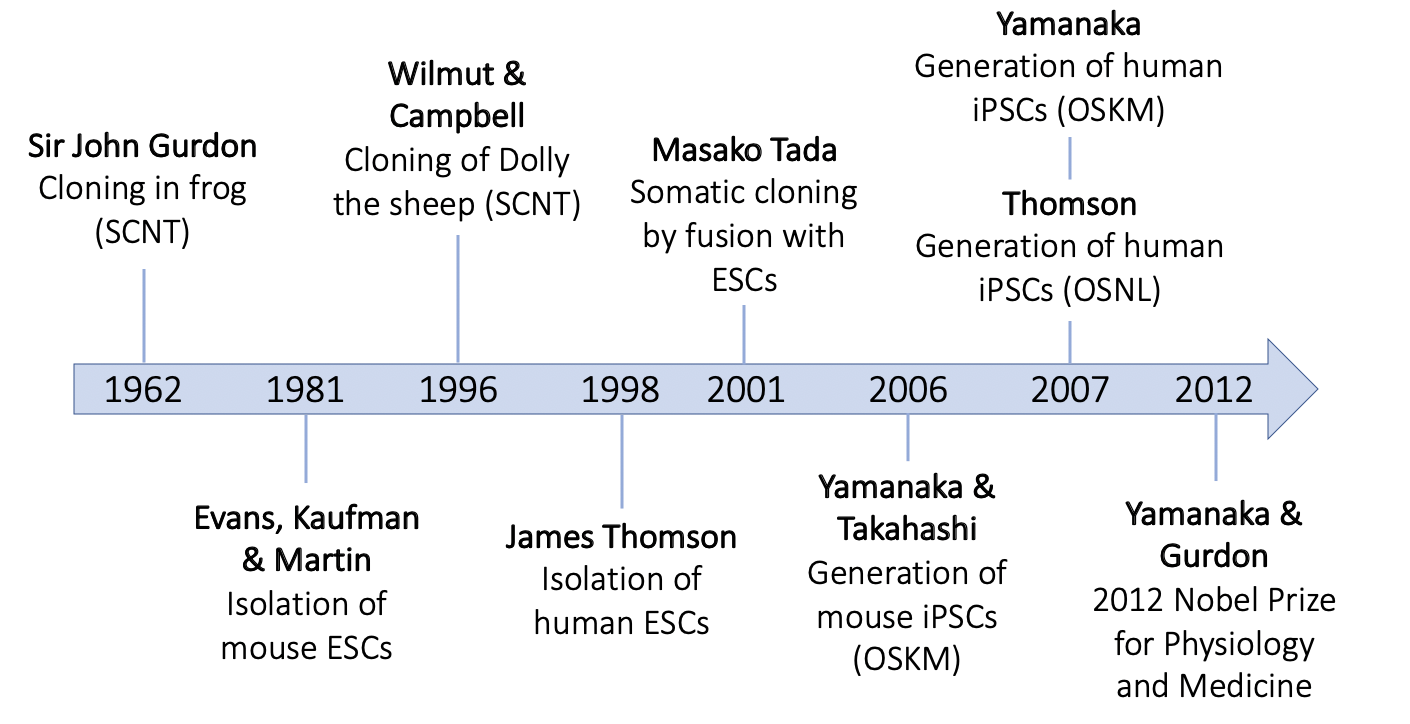
\includegraphics[width=15cm]{Chapter1/Fig/ipsc_timeline.png}
\caption[iPSCs timeline]{\textbf{Historical timeline of key events leading to the development of iPS cells}.\\
Key events including somatic cloning and isolation of ES cells that eventually led Shinya Yamanaka and colleagues to generate iPSCs in 2006 and Yamanaka to win the 2012 Nobel Prize for Physiology and Medicine alongside Sir John Gurdon.}
\label{fig:ipsc_timeline}
\end{figure}

\subsubsection{Inducing pluripotency}

The generation of \glspl{ipsc} involves the reprogramming of differentiated somatic cells from readily accessible tissue (such as skin or blood) into a pluripotent state by the introduction of a cocktail of factors to `reset' the transcriptional programme of the cell back to an embryonic state \cite{saha2009technical}. \\

The induction of iPSCs (in mice)
% induction of pluripotent stem cells from somatic cells was first demonstrated in mice in 2006.
was first described in 
a seminal paper published in \textit{Cell}.
In it, Takahashi and Yamanaka first demonstrated induction of pluripotent stem cells from both embryonic and adult mouse fibroblasts by inducing four transcription factors, Oct3/4\footnote{also called Pou5f1.}, Sox2, c-Myc and Klf4, under ES cell culture conditions \cite{takahashi2006induction}.

In the paper, the authors demonstrate that \glspl{ipsc} exhibited similar morphology, proliferation properties and doubling times compared to \glspl{esc}.
Additionally, iPSCs expressed major ES cell marker genes like \textit{SSEA-1} and \textit{Nanog} and formed teratomas upon injection into immunocompromised mice\footnote{A teratoma is a non-malignant tumor comprised of a disorganised mixture of cells from all three of the embryonic germ layers. 
In a teratoma assay, putative pluripotent stem cells are implanted into an immune-compromised mouse where they may proliferate and differentiate to form a teratoma. }.\\ 

However, these `first generation' \glspl{ipsc} failed to generate adult chimerae\footnote{A chimera is a single organism composed of cells with more than one distinct genotype.
The name derives from Greek mythology, where a chimera was a fire-breathing monster that was part lion, part goat, and part dragon. 
To generate a chimera, \gls{ips} cells (e.g. with a gene-specific mutation) are injected into blastocysts, which are then transplanted into the uteri of pseudo-pregnant mice.
By breeding a chimeric mouse with a wildtype mouse and observing the corresponding phenotype, e.g. coat colour, one can assess the contributions of the \glspl{ipsc} to the germline \cite{okita2007generation}.} or contribute to the germline \cite{takahashi2006induction}, suggesting that the \glspl{ipsc} were only partially reprogrammed \cite{omole2018ten}. 
In 2007, Yamanaka and other laboratories modified the induction protocols to generate fully reprogrammed `second generation' \glspl{ipsc} that were competent for adult chimera and germline transmission \cite{maherali2007directly, wernig2007vitro, okita2007generation}.\\

A year later, the Yamanaka and the Thomson labs demonstrated, at the same time, successful induction of pluripotent stem cells in human.
In the Yamanaka paper \cite{takahashi2007induction} human iPSCs were derived from adult human dermal fibroblasts using a retroviral system and the same 4 factors used in mice, which later became known as the Yamanaka factors: Oct3/4, Sox2, Klf4 and c-Myc (or OSKM).
On the same day, the Thomson group (the same group that had isolated human ESCs for the first time in 1998) also successfully generated human \glspl{ipsc}, using a slightly different technique: they used a lentiviral system to express the factors, and changed two of the inducing factors used: Oct4 and Sox2 remained, but the other two were replaced by Nanog and Lin28: this set of factors is sometimes called OSNL \cite{yu2007induced}.\\

In the next two years (2007-2009), the same technology was successfully applied by several groups and across a range of human cell types, including fibroblasts \cite{park2008reprogramming} but also other somatic cell types, such as pancreatic $\beta$ cells \cite{stadtfeld2008reprogramming}, neural stem cells \cite{eminli2008reprogramming, kim2008pluripotent}, stomach and liver cells \cite{aoi2008generation}, mature B lymphocytes \cite{hanna2008direct}, melanocytes \cite{utikal2009sox2}, adipose stem cells \cite{sun2009feeder} and keratinocytes \cite{maherali2008high}, demonstrating the universality of cellular reprogramming \cite{omole2018ten}.

% \newpage

\subsubsection{Challenges in the use of iPSCs}
Yet for \glspl{ipsc} to fulfil their promise (that they are viable and possibly superior substitutes for ESCs in disease modeling, drug discovery, and regenerative medicine), several challenges on the road to their clinical application needed to be overcome.
First, very low efficiency was recorded: in the original Yamanaka paper, only 0.01–0.1\% \cite{takahashi2006induction} of the starting cells effectively exhibited pluripotency, and other initial reports did not exceed 1\% \cite{takahashi2007induction, okita2007generation, lowry2008generation}.

Second, the over-expression of oncogenes (genes that have the potential to cause cancer) such as \textit{c-Myc} and \textit{Klf4} during the generation of \glspl{ipsc} raised safety concerns.
% The generation of iPSCs is not without challenges.
% % this may be wrong, near 100\% using Rais et al Nature 2013
% First, very low efficiency was originally recorded: 
% % in particular, on average, only 3-5\%\footnote{
% in the original Yamanaka paper, 
% % the percentage was even lower:
% 0.01–0.1\% \cite{takahashi2006induction}
% % .}  
% of the starting cells effectively exhibit pluripotency and can be used for further studies, and until 2011 the percentage was still as low as 3-5\% \cite{plath2011progress}.
% Efficiency has massively improved more recently, using a method described in \cite{rais2013deterministic}.
% By ... the efficiency can be as high as 50\% but with.. higher somatic mutation rate\\
Indeed, in the original report of germline-competent \glspl{ipsc}, $\sim$20\% of the offspring developed tumors attributable to the reactivation of the \textit{c-Myc} transgene \cite{okita2007generation}. 
Furthermore, there is the risk of insertional mutagenesis due to virus-based delivery methods \cite{takahashi2006induction, takahashi2007induction, yu2007induced}. 
Finally, several studies have reported incomplete reprogramming, with cells maintaining some degree of `epigenetic memory' from their somatic cell of origin, which can lead to their biased differential potential into certain cell types depending on the donor cell source \cite{kim2010epigenetic, polo2010cell}.\\

Much progress has been made in the past decade to address these limitations and to improve the reprogramming technique, including the development of new methods to induce reprogramming. 
In the following sections I present an overview of the advances made to improve the reprogramming technique, and discuss the reprogramming factors used and mechanisms of induction, the delivery system and the the somatic cell source chosen for iPSC generation.
Finally, I describe methods for characterising \glspl{ipsc} in general. 
\subsubsection{Reprogramming factors}

Generating \glspl{ipsc} requires the introduction of pluripotency related factors into the somatic cell. 
The generation of \glspl{ipsc} by Yamanaka’s and Thomson’s groups using different cocktails of transcription factors may suggest that different transcription factors activate the same reprogramming pathway by reinforcing each other’s synthesis.
As a consequence, apart from the `fantastic four' OSKM transcription factors, Sox2, Klf4, Oct4, c-Myc and the alternative combination described by the Thomson group containing Sox2, Oct4, Lin28 and Nanog (OSNL, \cite{yu2007induced}), other factors, sometimes referred to as `reprogramming enhancers', have been found to increase reprogramming efficiency and iPSC quality \cite{takahashi2016decade}.
Those include other transcription factors, small molecules, microRNA’s (miR) and different culturing conditions. 

% maybe add table here.
% \\

% The generation of \glspl{ipsc} by Yamanaka’s and Thomson’s groups using different cocktails of transcription factors may suggest that different transcription factors activate the same reprogramming pathway by reinforcing each other’s synthesis. The OSKM and OSNL reprogramming cocktails have proved efficient on a wide range of delivery systems, albeit at a variably low-efficiency rate (Gonzalez, Boue \& Izpisua Belmonte, 2011; Yakubov et al., 2010). 

% Consequently, researchers have sought to discover new molecules that will enhance the reprogramming technique and improve its efficiency (Table 2). We will refer to these molecules as reprogramming “enhancers.” 

Some other molecules have been discovered to act as `barriers' of reprogramming technique. 
% So the strategy employed to increase the efficiency of reprogramming includes the inhibition of such barriers and the over-expression and administration of the enhancers.

% Most factors have been found to target main cell signalling pathways including the TGF$\beta$, PI3K, $\beta$-catenin, cAMP and the MAPK/ERK pathways as well as apoptosis/cell cycle related pathways. 
% Furthermore, several factors that are known to be involved in chromatin remodelling pathways or in the hypoxia response pathway have also been reported to influence reprogramming. 
% Additionally, Glis1 as well as other genes of the Sox family (Sox1, Sox3, Sox15, Sox18), Klf family (Klf2, Klf1, Klf5) and Myc family (N-Myc, L-Myc)
% mir-302/367
% although with varying efficiencies.
% worth looking into which are commonly used now e.g. in HipSci

% add feeder-free here?

% Reprogramming enhancers
% Reprogramming barriers
% Cell cycle regulators
% Epigenetic modifiers

\subsubsection{Mechanisms of iPSC induction}
% \textbf{Technical aspects of iPSC induction}

% Oct4, Sox2, and Nanog bind together to activate the promoters of both their genes and those of each other, hence forming an autoregulatory loop. 
% The three factors function cooperatively to maintain their expression, thus enhancing the stability of pluripotency gene expression.\\

Several studies have described how the ectopic expression of OSKM in somatic cells induces the transition to a pluripotent state \cite{yamanaka2007strategies, brambrink2008sequential, stadtfeld2008induced, polo2012molecular, hansson2012highly, buganim2012single}. 
Based on these studies, we can now describe the order of events during the reprogramming process, which can be divided broadly into two waves or phases: an initial, stochastic early phase (phase 1) and a more deterministic and hierarchical late phase (phase 2) \cite{omole2018ten, takahashi2016decade, brouwer2016choices}.\\

% this may need more detail 
During induction using the OSKM factors, the first transcriptional wave (phase 1) is mostly mediated by c-Myc and occurs in all cells, whereas the second wave (phase 2) is more restricted to reprogrammable cells and involves a gradual increase in the expression of the Oct4 and Sox2 targets, leading to the activation of other pluripotency genes that aid in the activation of the pluripotency network. 
Klf4 seems to support both phases by repressing somatic genes during the first phase and facilitating the expression of pluripotency genes in the second phase \cite{buganim2013mechanisms}.\\

The two phases describe the mechanisms of reprogramming in the cells that successfully become pluripotent \glspl{ipsc}.
However, as we have seen, these are a rather small percentage of all transduced cells.
Three models, the elite, stochastic and deterministic models have been proposed to explain the reason behind such low reprogramming efficiency \cite{omole2018ten}.
For more detail into these three models, I refer the reader to Takahashi \& Yamanaka \cite{takahashi2016decade}.

\begin{figure}[htbp]
\centering
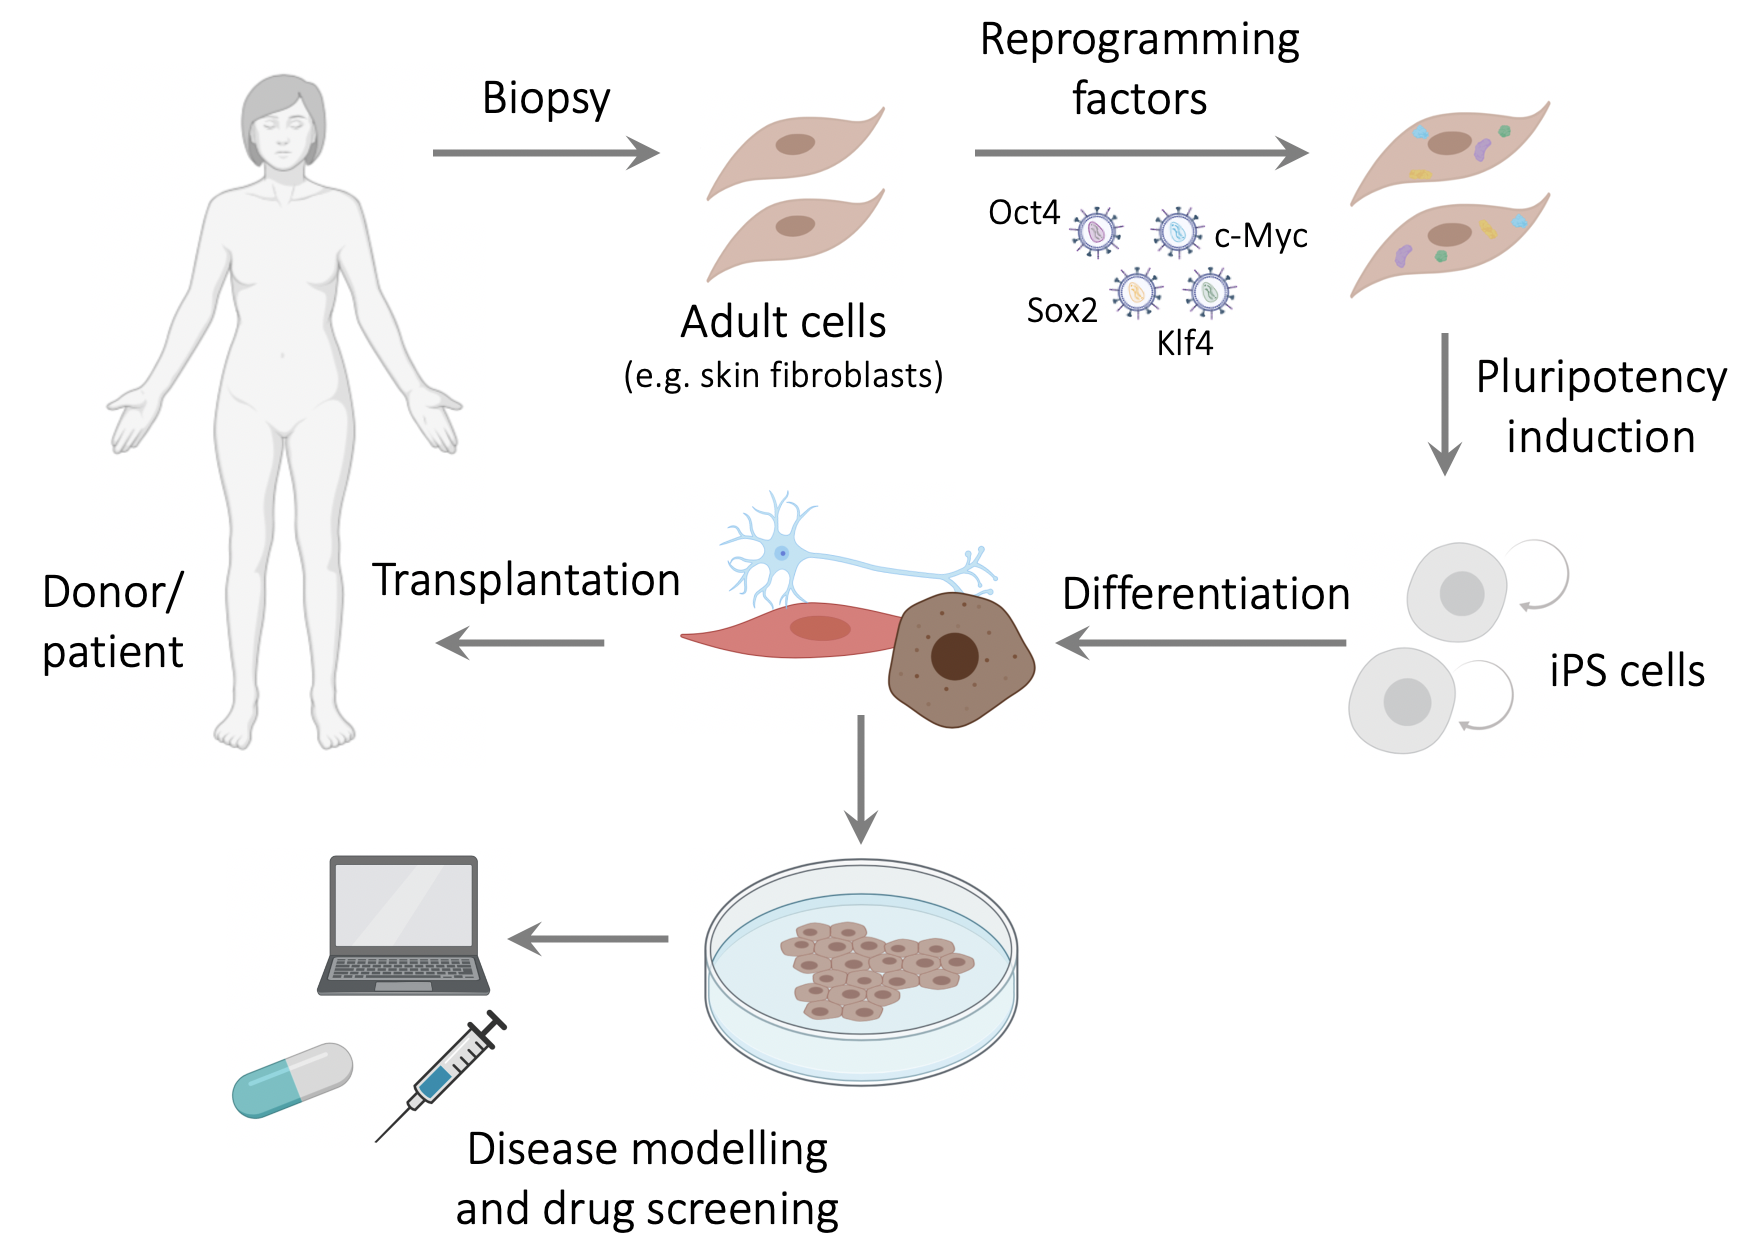
\includegraphics[width=14cm]{Chapter1/Fig/ipscs.png}
\caption[iPS cells]{\textbf{iPS cells - derivation and applications}.\\
The generation of iPSCs starts with a biopsy from, for example, the skin of an adult donor.
Adult cells, in the example fibroblasts, are then isolated and pluripotency is induced through four reprogramming factors, for example the Yamanaka factors: Oct4, Sox2, Klf4 and c-Myc (OSKM).
The factors can be delivered using a number of systems, see \textbf{section \ref{sec:ipsc_delivery}}.
The resulting induced pluripotent stem cells (iPSCs) are self-renewing and are virtually indistinguishable from ESCs.
They can be subsequently be differentiated towards other cell types, including disease relevant cell types, for example dopaminergic neurons for Parkinson's disease, or pancreatic beta cells for diabetes.
In the future, iPSC-derived cells might be used for cell therapy, i.e. they could be transplanted into the patient, with no risk of allogenic rejection.
In the meantime, iPSCs and iPSC differentiation can be used to model development and disease, and to do compound screening and drug testing.}
\label{fig:ipsc}
\end{figure}

\clearpage

\subsubsection{Delivery methods}
\label{sec:ipsc_delivery}

A number of different delivery methods have been used to introduce reprogramming factors into somatic cells. 
The reprogramming methods can be grouped into two categories: integrative systems (involving the integration of exogenous genetic material into the host genome) and non-integrative systems (involving no integration of genetic material into the host genome). \\

Early methods to deliver the reprogramming factors were integrative.
These include viral vectors (retrovirus \cite{takahashi2006induction, takahashi2007induction, wernig2007vitro, okita2007generation, yamanaka2007strategies, maherali2007directly}, lentivirus \cite{yu2007induced, blelloch2007generation}, and 
inducible and 
excisable retrovirus \cite{soldner2009parkinson} or
lentivirus \cite{maherali2008high}). 

Overall, integrative delivery methods have a higher reprogramming efficiency than non-integrating methods, but they are less safe due to the risk of insertional mutagenesis. \\

A major milestone in solving this issue was the introduction of efficient, integration-free methods for cell reprogramming. 
Alternative non-integrative induction methods have been developed that involve the transient expression of reprogramming factors, including the use of viral vectors (adenovirus \cite{stadtfeld2008reprogramming} and Sendai virus \cite{fusaki2009efficient, nishimura2011development}) and non-viral vectors, including plasmids \cite{yu2009human, okita2008generation, okita2011more, jia2010nonviral}, transposons \cite{kaji2009virus, woltjen2009piggybac, yu2009human} synthetic mRNAs \cite{warren2010highly} and recombinant proteins \cite{kim2009generation}. \\

Because they are safer, the use of non-integrating methods is overall more appealing for iPSC generation and use in a clinical setting.
Currently, episomal vectors, Sendai viruses and synthetic mRNAs are the most popular methods used for generating integration-free \glspl{ipsc}. 

% \textbf{Sendai}

% \textbf{plasmid}\\

% Additionally, induction is fairly robust to the system used to induce the factors: methods that have been used include i) viral transduction (retrovirus, lentivirus, Sendai virus), ii) DNA-based induction combined with plasmid transfection, iii) synthetic mRNA transfection and iv) recombinant proteins and protein tranduction \cite{narsinh2011comparison}.
% % PiggyBac Transposon, Episomal Vector Transfection,   
% % more ref: [71,72,73,74,75,76,77,78] from buganim

\subsubsection{Somatic cell of origin}

As for the cell source for reprogramming, somatic cells should preferentially be easily accessible, susceptible for reprogramming and the reprogramming process should ideally be highly efficient \cite{brouwer2016choices}. 
Many human somatic cell types have been successfully reprogrammed; however, reprogramming efficiencies and kinetics vary between somatic cell types. 
Keratinocytes for example showed a 100 times higher reprogramming efficiency ($\sim$0.8\%) and were reprogrammed two times faster than skin fibroblasts under the same conditions \cite{aasen2008efficient}. \\
% Furthermore, in mice it has been shown that immature cells are more readily reprogrammed than terminally differentiated cells \cite{eminli2009differentiation}. 

Today, human \glspl{ipsc} have been derived from a multitude of cell types \cite{doss2019current}, including dermal skin fibroblasts \cite{takahashi2007induction, yu2007induced}, adipocytes \cite{sugii2010human}, nucleated blood cells from peripheral blood \cite{loh2009generation, seki2010generation}, dental pulp \cite{yan2010ips},
keratinocytes from hair follicles \cite{aasen2008efficient} and
renal tubular cells from urine samples \cite{cao2018generation}.
However, approximately 80\% of human \glspl{ipsc} used in published studies are generated from fibroblasts \cite{takahashi2016decade}. \\
% potentially add epigenetic memory here

As mentioned above, the choice of cell source may also have consequences in terms of the epigenetic makeup of the \glspl{ipsc} generated.
Indeed, during the reprogramming process the somatic cells' epigenetic signature must be erased in order to adopt a stem cell-like epigenome.
These changes include chromatin reorganisation, DNA demethylation of promoter regions of pluripotency genes like \textit{NANOG}, \textit{SOX2} and \textit{OCT4}, reactivation of the somatically silenced X chromosome, and genome-wide resetting of histone post-translational modifications \cite{takahashi2007induction, maherali2007directly, wernig2007vitro, buganim2013mechanisms}.
If the reset is incomplete, cells may maintain some degree of `epigenetic memory' from their somatic cell of origin, which can lead to biased differential potential \cite{kim2010epigenetic, polo2010cell}.
% more references [62,63,64,65,66] from buganim
However, it has been shown that their residual epigenetic memory diminishes as the cells are passaged in culture over a period of time \cite{ghosh2010persistent}.
% \cite{omole2018ten, takahashi2016decade, brouwer2016choices}

\subsubsection{Characterising iPSCs}
\label{sec:ipsc_characterise}

As iPSC reprogramming efficiencies are low, it is important to carefully characterise the \glspl{ipsc} obtained after reprogramming \cite{brouwer2016choices}.
Different methods have been and should be used in combination to deeply characterise \glspl{ipsc}. 
% Morphology (flat, tightly packed)
First, the characteristic ES-like morphology of \glspl{ipsc} is often used as an indication of their correct formation. 
\glspl{ipsc} can be observed as small cells with large nucleus/cytoplasm ratios that form tightly packed colonies with clear, sharp edges. 
Second, \glspl{ipsc} are characterised by the expression of pluripotency markers including Oct4, Nanog, SSEA-3, SSEA-4, TRA-1-60 and TRA-1-81 \cite{boulting2011functionally}.
Additionally, bioinformatics tools, such as the PluriTest \cite{muller2011bioinformatic}, have been developed which use gene expression to assess the level of pluripotency. \\

% Pluripotency markers (Alkaline phosphatase assay, Expression of pluripotency markers: Oct4, Nanog, SSEA3/4, Tra-1-60, Tra-1-81 
In addition to morphological and gene expression considerations, \glspl{ipsc} can also be evaluated functionally by their differentiation potential.
Indeed, \glspl{ipsc} should be able to terminally differentiate into cells of all three germ layers (endoderm, mesoderm, ectoderm) - which can be evaluated through \textit{in vivo} teratoma formation assays or \textit{in vitro} differentiation through embryoid body (EB) formation.
Finally, since reprogramming influences the genetic and epigenetic make-up of the cells, \glspl{ipsc} should be carefully characterised for their genetic and epigenetic profiles.
Specifically, karyotyping is commonly used to evaluate genetic abnormalities in \glspl{ipsc}, i.e. to verify that cells are diploid. 
Additionally, if transgenes are used for reprogramming, it is important to verify that the expression levels of the transgenes are properly down regulated once the \glspl{ipsc} are formed. 
As for the evaluation of the epigenetic profile of the \glspl{ipsc}, DNA methylation patterns can be assessed. 
Since DNA methylation contributes to silencing of genes, it is important that the generated \glspl{ipsc} show DNA demethylation at key pluripotency genes (e.g., \textit{Oct4, Nanog, Sox2}), while genes specific to the donor somatic cell type become methylated and silenced \cite{brouwer2016choices, omole2018ten}. 

% Still, challenges remain in the generation of \glspl{ipsc}.
% % this may be wrong, near 100\% using Rais et al Nature 2013
% Besides the low efficiency which is only partially improved by added molecules and changed culture conditions, tumorigenicity and epigenetic memory.\\

% \textbf{Tumorigenicity of iPSCs}\\
% % expand on mutations and tumorigenicity
% % It has been shown that mutations can be accumulated during the reprogramming process.
% % Genomic insertions ...
% % the initial methods for iPSC derivation employed genome-integrating retroviral/lentiviral vectors, which could produce tumorigenic insertional mutations. 
% % simplify this sentence
% % i) good to model tumours
% % ii) dangerous for cell replacement
% % iii) trade-off cancer vs efficiency
% One of the major issues with the use of iPSC for potential cell replacement therapy is the risk of potential tumorigenicity from undifferentiated \glspl{ipsc} in the cell population that will be used for cellular transplantation. 
% The key concept is that \glspl{ipsc} will almost certainly never be used in regenerative medicine if they are not able to cause a teratoma in mice [18,83,84]. 
% \glspl{ipsc} can form both teratomas and malignant tumors such as neuroblastoma and follicular carcinoma if transplanted in their undifferentiated pluripotent state \textit{in vivo} [84]. 
% Thus, the potential tumorigenicity risk to human patients from both teratomas and malignant tumors is quite possible if transplanted cells are contaminated with undifferentiated \glspl{ipsc}. 

% Tumorigenicity has been observed, and only partially solved by removing the oncogene c-Myc.
% In fact, inactivation or deletion of the tumor suppressor p53, which is a key regulator of cancer, significantly increases reprogramming efficiency \cite{marion2009p53}.
% Thus there seem to be a trade off between cancer inducing and efficient reprogramming.\\

% \textbf{Epigenetic memory}\\
% % summarise epigenetic memory
% Finally, several studies have reported incomplete reprogramming, with cells maintaining some degree of `epigenetic memory' from their somatic cell of origin, which can lead to their biased differential potential into certain cell types depending on the donor cell source \cite{kim2010epigenetic, polo2010cell}.
% % more references [62,63,64,65,66] from buganim
% This is due to incomplete resetting of the somatic cells' epigenetic signature,which must be erased during reprogramming in order to adopt a stem cell-like epigenome. 
% These changes include chromatin reorganisation, DNA demethylation of promoter regions of pluripotency genes like \textit{Nanog}, \textit{Sox2} and \textit{Oct4}, reactivation of the somatically silenced X chromosome, and genome-wide resetting of histone post-translational modifications \cite{takahashi2007induction, maherali2007directly, wernig2007vitro, buganim2013mechanisms}.

% However, it has been shown that their residual epigenetic memory diminishes as the cells are passaged in culture over a period of time \cite{ghosh2010persistent}.
% % [67,68] from. buganim

% % expand XCI
% One more note on X chromosome inactivation (XCI).
% \glspl{ipsc} are heterogeneous due to random X inactivation in cell lines derived from female individuals.

% Here, we have studied genome-wide expression profiles of multiple new and existing hiPSC lines and shown that the XCI marker XIST RNA can be used as a readout to assess one aspect of female hiPSC quality.
% We therefore encourage the use of XCI markers as a benchmark to assess quality of all female h\glspl{ipsc}.
% \cite{anguera2012molecular, bar2019global}

% Third, most of the derivation and culture of human \glspl{ipsc} employed undefined human ESC culture media and feeder cells.

% \cite{halevy2014comparing, park2008reprogramming, doss2019current}

\subsubsection{Heterogeneity of iPSCs and between cell line variation}

An important aspect of iPSC biology is the  large variability observed between different iPSC lines and clones (even when derived from the same donor). 
This includes differences
% Given the huge variability across iPSC lines and their differentiated derivatives 
in terms of their differentiation potential, epigenetic status, tumorigenic potential, immunogenic potential, maturation characteristics, batch variability and co-occurrence of heterogenous populations of lineage subtypes and/or non-relevant cells as contaminating cell populations \cite{buganim2013mechanisms}.
This observed diversity, which is greater than what has been described in ESCs, can be explained by the residual epigenetic memory, genetic background and the characteristics acquired during reprogramming and differentiation \cite{kim2010epigenetic, polo2010cell, rouhani2014genetic}.
Naturally, understanding these sources of variable differentiation, particularly in terms of efficacy and safety, will be critical for the successful use of cell replacement therapies in the clinical setting \cite{buganim2013mechanisms}. \\

Thus, it is important to investigate sources of variable differentiation potential across lines, including lines derived from genetically distinct individuals.

% \subsubsection{Differentiating iPSCs}

% In order to induce differentiation of \glspl{ipsc} to whatever fate we might need one must mimick the signalling pathways that are activated \textit{in vivo}.
% % This is challenging as it involves temporal and spatial considerations.

% Whilst many protocols have been established in the last decade which allow generation of iPSC-derived heart cells, liver cells, blood cells and many others, I will here highlight briefly the key steps and genes involved for the two protocols we used in work I present in this thesis: definitive endoderm and midbrain dopaminergic neurons.\\

% \textbf{Definitive endoderm}

% % this needs detail
% The endoderm is the innermost of the three germ layers\footnote{from the greek endo for inner, as opposed to meso: middle and ecto: outer.}.
% It gives rise to the gastro-intestinal duct (esophagus, small and large intestine) and related organs (liver, pancreas) as well as to the pulmonary system (lungs).
% As we have seen, it is during gastrulation that the three layers are formed.\\

% The process to generate endoderm cells involves first inducing a mesendoderm fate, where cells are bipotent for either mesoderm or endoderm.
% To achieve this, we need to suppress the expression of pluripotency markers such as \textit{NANOG} and \textit{OCT4} and encourage the expression of master regulators of the mesendoderm, such as \textit{NODAL} and \textit{T} (Brachiury).
% % To do so, ..\

% Second, to induce the endoderm specifically, the expression of \textit{CXCR4} and \textit{GATA6} is encouraged.\\

% % \newpage

% \textbf{Dopaminergic Neurons}
% % this needs cleaning up too

% % from Gioele La Manno's thesis
% % The molecular description of the steps through which these progenitors cells generate uniquely fated neurons and glia is one of the primary goals of developmental neurobiology (Brody and Odenwald, 2005).

% The central nervous system (CNS) is formed at the end of gastrulation from ectoderm cells under the influence of SHH, an inductive factor derived from the notochord.
% In the process of neurulation the neural tube is formed as a results of the folding of the neural plate, as mediated by BMP signalling \cite{grove2013comprehensive}. 
% Cells called organisers, such as the floor plate, provide an initial patterning of the neural tube into forebrain (cortex), midbrain and hindbrain.
% % The ventral midbrain is a part of the brain whose development has been extensively studied, particularly in connection to Parkinson’s disease, the second most common neurodegenerative pathology after Alzheimer’s. 
% % Parkinson’s disease is named after the 19th century physician, James Parkinson, that first described its symptoms: tremor, bradykinesia, rigidity and postural instability (Parkinson, 2002).
% % Only a century later the disease was characterised histopathologically, by Frederic Lewy, and was found to be caused by the progressive death of dopaminergic neurons in the substantia nigra pars compacta (Holdorff, 2002).
% % Interest in the details of dopaminergic lineage development is fostered by the possibility that knowledge of this process could help to develop new therapies for Parkinson’s disease. Current treatments for Parkinson’s disease alleviate the symptoms but fail to address the cause of the disease. At the moment, arresting or effectively slowing down the progression of the disease is not possible. In this context, alternative therapeutic approaches that aim at the regeneration or replacement of degenerated neurons are being explored. In particular, cell- replacement therapies using human mesencephalic fetal tissue have shown promising initial results in clinical trials (Lindvall and Kokaia, 2009). The approach is currently being refined and further investigated through more extensive trials (Barker et al., 2015). However, to guarantee the safety and reproducibility required for clinical adoption, cells must be derived from standardised, easily accessible and scalable sources. To this purpose, patient-derived induced pluripotent stem cells (iPSC) or embryonic stem cells (ESC) have been envisioned as the best alternative, supported by evidence that these cells can differentiate into dopaminergic neurons (Arenas et al., 2015).
% % The path that leads to safer and more effective cell-replacement therapy passes through the acquisition of a more detailed picture of midbrain development. This knowledge will not only help to assess how similar in vitro cells are to their in vivo counterparts, but also to learn how to recapitulate in vivo differentiation.
% % Ventral midbrain development has been thoroughly studied in mice. After neurulation, three important organisers of the midbrain are formed: the floor plate, the dorsal midline and the midbrain-hindbrain boundary. These floor plate is generated as the result of SHH, a morphogen initially synthesised by the notochord (and later by the floor plate). The midbrain- hindbrain boundary is formed by expression of two transcription factors OTX2 (anterior) and GBX2 (posterior) (Figure 5) and, together with the dorsal midline, secretes two morphogens essential for ventral midbrain development: FGF8 and WNT1 (Nakamura, 2013).
% % Midbrain dopaminergic neuron development is triggered within the floor plate by the expression of Lmx1a, a target of OTX2, and the activation of the beta catenin pathway in response to WNT1 signaling (Chung et al., 2009). More laterally, where the level of SHH is low, the basal plate program is triggered instead (Figure 4) (Prakash et al., 2009).

% % Further steps leading to the development of dopaminergic neurons have been characterised and involve the successive activation of key transcription factors such as Nr4a2 and Pitx3. In contrast, bifurcation events leading to the segregated dopaminergic populations of the substantia nigra and ventral tegmental area are less well understood, despite the implication for Parkinson’s disease, in which substantia nigra neurons degenerate (Damier et al., 1999).
% % The differentiation between the substantia nigra and ventral tegmental populations has motivated efforts to count the populations of dopaminergic neurons that populate the midbrain. This work has expanded the classification from two fundamental types to more; for example, a classification based on connectivity and electrophysiological recording arrived at 13 dopaminergic populations (Roeper, 2013). Attempts to molecularly profile different populations distinguished fewer types (Chung et al., 2005). The most recent example of these attempts used single-cell real-time PCR profiling of a curated gene set to discover five dopaminergic neuron populations in the adolescent mouse (Poulin et al., 2014).
% % This discrepancy between the numbers of phenotypically and molecularly defined cell types is just another reminder of the necessity for systematic and unbiased molecular characterisation of these types. Furthermore, in a panorama where molecular details were mainly studied in mice and chicken embryos, profiling of human development could have a critical translational impact. The knowledge of similarities and peculiarities might turn out to be essential in improving current differentiation protocols for cell-replacement therapies.

% % The notochord secretes molecules to neuronal stem cells, often called neuronal progenitor cells (NPCs).  
% % The level along the notochord (most cranial, middle, most caudal) will determine what type of neuronal cells the NPCs will produce: they will become the forebrain, midbrain and hindbrain, respectively.
% % This is known as patterning?

% FGF8 (DA)
% FGF4 (Sert)

% Dopaminergic and serotonergic neurons are part of the substantia nigra (literally black matter), which is part of the midbrain.

% Towards the end of neurogenesis (week XX), the NPCs start to produce another (non-neuronal) type of cells.
% Those are glia cells, and include oligodendrocytes, astrocytes and ependymal cells.


% In particular, neurogenesis (generation of neurons) begins at around week 5 ($\sim$ day 11).

% %********************************** % 1.2.1  **************************************
% \subsection{Clinical applications of human stem cells}
% \label{sec:human_stem_cell_applications}

% The promise of induced pluripotent stem cells in research and therapy \cite{robinton2012promise}

% first human embryonic stem cells (ESCs) based model (a model for Lesch-Nyhan syndrome by targeting of the HPRT gene in human ESCs)\cite{urbach2004modeling}
% \cite{halevy2014comparing}

% other models were further used to obtain novel mechanistic or physiological insights regarding the disorders. One example is a model for Amyotrophic Lateral Sclerosis (ALS) by Kiskinis et al \cite{kiskinis2014pathways} \\


% \textbf{mouse iPSCs} (paragraph from Saha and Jaenish 2009 \cite{saha2009technical}):
% Recent work with rodents has tested the developmental potential of \glspl{ipsc} and their potential for the treatment of diseases. 
% Differentiation of mouse \glspl{ipsc} can be directed in vitro into cardiovascular (Kuzmenkin et al., 2009; Narazaki et al., 2008; Schenke-Layland et al., 2008), hematopoietic (Hanna et al., 2007; Schenke-Layland et al., 2008; Xu et al., 2009), neural (Wernig et al., 2008), and hepatic progenitor cells (Cantz et al., 2008), and recently, mouse \glspl{ipsc} passed the most stringent test of pluripotency by generating full-term adult mice in tetraploid complementation assays (Boland et al., 2009; Kang et al., 2009; Zhao et al., 2009). 
% Further, mouse \glspl{ipsc} obtained from adult fibroblasts can be used to restore physiological function of diseased tissues in vivo, as demonstrated by using iPSC-derived hematopoietic cells in a humanised mouse model of sickle cell anemia (Hanna et al., 2007). 
% Also, endothelial/endothelial progenitor cells derived from mouse \glspl{ipsc} injected directly into the liver of irradiated hemophilia A mice extended their survival for more than 3 months and rescued depleted Plasma FVIII levels (Xu et al., 2009). Finally, functional dopamine neurons could be generated from reprogrammed mouse fibroblasts, and transplantation of these neurons, like mESC-derived neurons, could restore dopamine function when grafted into Parkinsonian rats (Wernig et al., 2008). These studies establish that \glspl{ipsc} have vast potential to generate a variety of functional cell types and can be used to modify the course of disease in rodents.\\

% \textbf{human iPSCs} (paragraph from Saha and Jaenish 2009 \cite{saha2009technical}):
% Differentiation of h\glspl{ipsc} into several cell types has already been achieved: neural progenitors (Chambers et al., 2009), motor neurons (Dimos et al., 2008; Ebert et al., 2009), dopaminergic neurons (Soldner et al., 2009), retinal cells (Osakada et al., 2009), hepatocytes (Sullivan et al., 2009), blood cells (Choi et al., 2009; Ye et al., 2009), adipocytes (Taura et al., 2009), endothelial cells (Choi et al., 2009; Sullivan et al., 2009), and fibroblasts (Hockemeyer et al., 2008; Maherali et al., 2008). 





% feeder: inactivated embryonic fibroblasts

% feeder-free is cheaper quicker more ethical

% teratoma assay to assess pluripotency.
% A teratoma is a non-malignant tumour that contains a mixture of cells from all three germ layers.
% \glspl{ipsc} or hESCs can be injected into an immuno-suppressed mouse and then we can wait until the mouse develops a teratoma and perform histological analysis of it to check that all layers (ecto, meso and endodermal cells) are present.




% \subsubsection{tissues and diseases}

% \textbf{Nervous system.}
% Disease-specific iPSC-derived neurons are also being used as in vitro models to elucidate the cellular and molecular pathogenesis of Parkinson disease83,84,85,86,87, Alzheimer disease88,89, ALS90,91,92,93, spinal muscular atrophy94,95 and others.


% \begin{itemize}
%     \item ESCs (embryonic stem cells)
%     \item TSPSCs (tissue-specific progenitor stem cells)
%     \item MSCs (mesenchymal stem cells)
%     \item UCSCs (umbilical cord stem cells)
%     \item BMSCs (bone marrow stem cells)
%     \item \glspl{ipsc} (induced pluripotent stem cells)
% \end{itemize}

% list from \cite{mahla2016stem}


% add timeline from (Current status of pluripotent stem cells: moving the first therapies to the clinic,  figure 2)

% \cite{kimbrel2015current}

% aurologous vs allogenic (ESCs are genetically different from receiver) transplant

% \subsubsection{ESCs vs iPSCs}

% Additionally, potential clinical use of autologous hiPSCs might not be hindered by immunological problems inherent to allogeneic hESC-derived cells. 

% genetic variation
% genome editing in ESCs not very efficient
% much easier to derive iPSCs with a given genetic background

% obvious ethical concerns and limitations (e.g. some countries might ban studies using ESCs altogether)

% most famous clinical application of stem cells is in laeukemia patients
% cells grow uncontrollably and prevent hematopoietic stem cells to proliferate so you can kill them with chemo/radio therapy and then transplant hematopoietic SCs back in (stem cell therapy?)

% In March 2017 a team led by Masayo Takahashi completed the first successful transplant of iPS-derived retinal cells from a donor into the eye of a person with advanced macular degeneration.[91] 

% %********************************** % 1.2.1  **************************************
% \subsection{iPSC consortia}

\subsection{Applications of human iPSCs in genetics}
\label{sec:ips_genetics}

In contrast to ES cells, the use of which, as we have seen, raises important ethical concerns\footnote{as it involves the destruction of the embryo}, iPSCs
% In order to obtain an ES cell one must destroy the embryo, raising ethical concerns that caused the generation of ESCs to be reduced substantially or even made illegal in some countries.
% In contrast, iPSCs 
can be derived from easily accessible tissues such as blood or skin, bypassing all such concerns.
Because they are fairly easy to derive, they can be generated for individuals from all genetic backgrounds, including individuals carrying a genetic disorder of interest.
In the future, the iPSC technology opens the way to regenerative medicine where tissues can be re-generated with one's own cells thus avoiding the risk of immune rejection (when the body rejects a donor's allogenic organ as a foreign object).\\

In addition to genetic disorders and tissue regeneration, the iPSC technology can be applicable to basic biological research of human development and disease modeling.
Indeed, human \glspl{ipsc} have already been differentiated into a plethora of differentiated cell types, including
% ectoderm
neural stem cells \cite{d2014large}, 
cortical, dopaminergic 
% (Ma et al 2011) 
and motor neurons \cite{shi2012human, kriks2011dopamine, karumbayaram2009directed},
astrocytes \cite{shaltouki2013efficient} and
oligodendrocytes \cite{douvaras2014efficient} 
as well as
% mesoderm
cardiomyocytes \cite{burridge2014chemically}, 
skeletal muscle cells \cite{maffioletti2015efficient}, 
vascular endothelial/smooth muscle cells \cite{patsch2015generation}, 
% endoderm
hepatocytes (liver cells) \cite{si2010highly},
pancreatic beta cells \cite{zhang2009highly} and 
lung epithelial cells \cite{huang2014efficient}.\\
% retina?

In recent years, as the iPSC technology became more established, iPSC lines have been derived from large cohorts of individuals, allowing deeper characterisation of these cells across multiple individuals.
This paved the way to the study of how common genetic variants affect gene expression in \glspl{ipsc}.
These large cohorts represent a resource which allows differentiation of a number of these lines and the interrogation of \glspl{eqtl} in derived differentiated cell types, too.

\subsubsection{HipSci and other human iPSC consortia}
% \textbf{HipSci}

The \gls{hipsci} is the largest human iPSC cohort to date, and the results described in this thesis are all obtained using data from \gls{hipsci} \cite{kilpinen2017common}.
The goal of \gls{hipsci} was to generate a large, high quality reference panel of human iPSC lines for the research community to help deeply characterise these cells. 
All \gls{hipsci} donors are volunteers from the Cambridge area in the UK. 
Donors are for the vast majority of European descent, both male and female and across a range of ages (for healthy donors, [50-54]-[65-69]).
The majority of lines are derived from healthy donors, with small groups of diseased\footnote{Diseases included in \gls{hipsci} are monogenic diabetes, Bardet-Biedl syndrome, Usher syndrome, Hypertrophic cardiomyopathy and a few others, see \url{http://www.hipsci.org}.} samples.
For sample collection, primary fibroblasts from skin biopsies (from the inner upper arm to minimise somatic mutations due to sun exposure) were collected from consented research volunteers recruited from the NIHR Cambridge BioResource and iPS cell derivation was performed either using the Sendai reprogramming kit or episomal plasmids expressing the (human) Yamanaka factors: human (h)OCT3/4, hSOX2, hKLF4 and hMYC \cite{yu2009human}.
Following transfer to feeder free culture and expansion, each line was submitted to quality control and the criteria for line selection were: (i) level of pluripotency, as determined by the PluriTest assay \cite{muller2011bioinformatic}; (ii) number of copy number abnormalities; and (iii) ability to differentiate into each of the three germ layers \cite{kilpinen2017common}. \\

% Medium:

% Transduced cells were culture on an irradiated mouse embryonic fibroblast (MEF-CF1) feeder
% picked between day30 and 40 and cultured in iPS cell medium until ready to passage (define). 
% Cells passaged every 5-7 days until established (usually at passage 5 or 6)
% then lines expanded for banking and characterisation
% now transferred to feeder-free culture
% % from 
% \cite{kilpinen2017common}.\\


% \textbf{other iPSC consortia and large studies}
Additional iPSC consortia and large studies include
iPSCORE (a panel of fibroblast-derived iPSC lines from 222 ethnically diverse and sometimes related individuals \cite{panopoulos2017ipscore}), GENESiPS (a collection of 317 peripheral blood mononuclear cell (PBMC)-derived iPSC lines from 101 individuals \cite{carcamo2017analysis}), PHLiPS (containing PBMC-derived iPSC lines from 91 individuals of European and African-American ethnicity \cite{pashos2017large}), and Banovich \textit{et al} (a cohort of 58 lymphoblastoid cell line (LCL)-derived Yoruban lines, \cite{banovich2018impact}).

\subsubsection{eQTL mapping using iPSCs and iPSC-derived cells}

In 2017, the \gls{hipsci} consortium published a first paper, where they assessed iPSC lines through various assays, and mapped \glspl{eqtl} in 711 cell lines from 301 unique donors \cite{kilpinen2017common}.
At around the same time, another map of iPSC \glspl{eqtl} was published in \textit{Cell Stem Cell} \cite{deboever2017large}.
% \cite{warren2017induced}
Most recently, a meta-study was published as the result of an effort to combine iPSC resources into the i2QTL consortium \cite{bonder2019systematic}.\\
% summarise main findings and numbers\\

Collectively, these studies have identified iPSC-specific eQTL, i.e. eQTL that function primarily in pluripotent cells.
A subset of these tagged disease-associated loci, suggesting that they are capturing molecular changes early in development which are not well captured by studies of differentiated primary tissues from adult individuals. 
Alternatively, iPSC eQTL may be capturing stem-cell like molecular mechanisms, which are similar to mechanisms active in cancer \cite{kilpinen2017common}. \\


In the last few years, \glspl{eqtl} have also been mapped in several iPSC-derived cell types.
These include iPSC derived-
macrophages \cite{alasoo2018shared},
hepatocytes \cite{pashos2017large},
neurons \cite{schwartzentruber2018molecular}
and
cardiomyocytes \cite{strober2019dynamic, banovich2018impact}.\\
% other?

These \glspl{eqtl} promise to greatly improve our understanding of genetic regulation in cell types that we do not typically have access to, including cells at developmental stages and cells that are difficult to isolate, such as neuronal cell types.
Combined with \gls{gwas} results, they can contribute to our understand of the genetic architecture of complex disease by facilitating analyis in the relevant cell types, for example dopaminergic neurons for Parkinson's disease (\textbf{Chapter
\ref{chapter5}})
% 5)
or endoderm-derived (\textbf{Chapter 
\ref{chapter4}})
% 4)
pancreatic beta cells for diabetes.

% add one concluding sentence/paragraph.

\newpage

\section{Thesis outline}

% In this thesis, I present novel and efficient LMMs that can model relationships between multiple variants and traits, and describe an inference framework that enables LMMs to be built flexibly.

% In this thesis, I describe new methods and applications for eQTL mapping using single cell expression profiles.

% The overarching topic of this thesis is the identification and interpretation of cell type and context-specific eQTL as detected using matched genotype information and expression profiles measured by \gls{scrnaseq}, across several individuals.\\

The overall aim of this thesis is to provide suitable computational methods for the identification of cell type and context-specific eQTL using single cell expression profiles, 
% and matched genotype information, 
and explore their application across a range of human iPSC-derived cell types, using data from the \gls{hipsci} project.\\

% The overall aim of this thesis is to provide suitable methods to perform \gls{eqtl} mapping using \gls{scrnaseq} expression profiles, and to explore the effects of common genetic variants on single cell expression across a range of human \gls{ipsc}-derived cell types using data from the \gls{hipsci} project.\\

% \newpage

Specifically, in \textbf{Chapter 
% 2
\ref{chapter2}}, I give an overview of current \glspl{lmm} for genetic analyses, covering their use for association and interaction testing, focusing on their application in \gls{eqtl} mapping.\\

In \textbf{Chapter 
% 3
\ref{chapter3}}, I describe best-practice approaches to perform \gls{eqtl} mapping using \gls{scrnaseq} profiles and demonstrate these methods on matched bulk and single cell expression of around 100 human \gls{ipsc} lines as well as on simulated data.  \\

In \textbf{Chapter 
% 4
\ref{chapter4}}, I present a dataset of almost 40,000 cells from 125 human \gls{ipsc} lines differentiating to definitive endoderm, and demonstrate different approaches to \gls{eqtl} mapping using \gls{scrnaseq} data, identifying genetic variants that affect gene expression dynamically along differentiation and across other cellular states. \\

In \textbf{Chapter 
% 5
\ref{chapter5}}, I present a dataset of over 1 Million cells from 215 human \gls{ipsc} lines to midbrain dopaminergic neurons.
We identify thousands of \glspl{eqtl} across a number of cell types and upon external stimulation.
In addition, we identify hundreds of colocalisation events with variants that are known to be associated with neurological traits and diseases.
Moreover, we investigate sources of variation in the capacity of individual cell lines to differentiate toward neurons.\\

% In \textbf{Chapter 
% % 6
% \ref{chapter6}}, I present a novel method to jointly test for context-specific \glspl{eqtl} across multiple cell types and states defined at single cell resolution, and show some preliminary results on single cell \gls{ipsc} data. \\

Finally, in \textbf{Chapter 
% 7
\ref{chapter7}} I conclude and discuss future directions.